%%%%%%%%%%%%%%%%%%%%%%%%%%%%%%%%%%%%%%%%%
% Beamer Presentation
% LaTeX Template
% Version 1.0 (10/11/12)
%
% This template has been downloaded from:
% http://www.LaTeXTemplates.com
%
% License:
% CC BY-NC-SA 3.0 (http://creativecommons.org/licenses/by-nc-sa/3.0/)
%
%%%%%%%%%%%%%%%%%%%%%%%%%%%%%%%%%%%%%%%%%

%----------------------------------------------------------------------------------------
%	PACKAGES AND THEMES
%----------------------------------------------------------------------------------------

\documentclass{beamer}

\newcommand{\EMSE}{ {\rm EMSE}}
\newcommand{\CC}{ {\rm CC}}
\newcommand{\MSE}{ {\rm MSE}}
\newcommand{\WIN}{\scriptscriptstyle {\rm WIE}}
\newcommand{\OROI}{\scriptscriptstyle {\rm out ROI}}
\newcommand{\Her}{\scriptscriptstyle H}
\newcommand{\T}{\scriptscriptstyle T}
\newcommand{\LMS}{\scriptscriptstyle {\rm LMS}}
\newcommand{\RDE}{\scriptscriptstyle {\rm RDE}}
\newcommand{\MRD}{\scriptscriptstyle {\rm MRD}}
\newcommand{\MSD}{\scriptscriptstyle {\rm MSD}}
\newcommand{\SBD}{\scriptscriptstyle {\rm SBD}}
\newcommand{\SDD}{\scriptscriptstyle {\rm SDD}}
\newcommand{\WIE}{\scriptscriptstyle {\rm WIE}}
\newcommand{\R}{\scriptscriptstyle {\rm R}}
\newcommand{\I}{\scriptscriptstyle {\rm I}}
\newcommand{\mT}{\scriptscriptstyle -T}
\newcommand{\vir}{,\hspace{-0.15ex}}
\newcommand{\M}{\scriptscriptstyle M}
\newcommand{\MMA}{\rm \scriptscriptstyle MMA}
\newcommand{\neigh}{\scriptscriptstyle {\rm neigh}}
\newcommand{\st}{\scriptscriptstyle {\rm st}}
\newcommand{\nd}{\scriptscriptstyle {\rm nd}}
\newcommand{\CSD}{\scriptscriptstyle {\rm CSD}}
\newcommand{\E}{{\rm E}}
\newcommand{\uM}{{\mathbf u}}
\newcommand{\rM}{{\mathbf r}}
\newcommand{\xM}{{\mathbf x}}
\newcommand{\yM}{{\mathbf y}}
\newcommand{\XM}{{\mathbf X}}
\newcommand{\w}{{\mathbf w}}
\newcommand{\wo}{{\mathbf{w}}_{\rm o}}
\newcommand{\q}{{\mathbf q}}
\newcommand{\qp}{{\mathbf {\dot{q}}}}
\newcommand{\Nuquad}{\|{\mathbf u(n)}\|^2}
\newcommand{\NuquadP}{\|{\mathbf u(n)}\|^2_{{\mathbf R}^{-1}(n)}}
\newcommand{\uMc}{{\mathbf u}^{\ast}}
\newcommand{\wtil}{\widetilde{\mathbf w}}
\newcommand{\Dw}{\boldsymbol{\Delta}{\mathbf w}}
\newcommand{\Dewp}{\boldsymbol{\Delta}{\mathbf{\dot{w}}}}
\newcommand{\Pb}{{\mathbf R}^{-1}}
\newcommand{\ebari}{{\bar{e}}_i}
\newcommand{\field}[1]{\mathbb{#1}}
\newcommand{\re}{\field{R}}
\newcommand{\co}{\field{C}}
\newcommand{\CO}{\field{C}}
\newcommand{\RE}{\field{R}}
\newcommand{\Tr}{{\rm Tr}}
\newcommand{\Ru}{{\mathbf R}}
\newcommand{\sgbeta}{\sigma_{\scriptscriptstyle{\!\alpha}}^2}
\newcommand{\sgphi}{\sigma_{\scriptscriptstyle{\!\varphi}}^2}
\newcommand{\cred}{\textcolor{red}}
\newcommand{\lbo}{\lambda_{\rm o}}
\newcommand{\cond}{\mathbf{w}_1(n\!-\!1),\mathbf{w}_{2}(n\!-\!1)}
\newcommand{\cb}{\textcolor{blue}}
\newcommand{\pu}{\mathbf{p}_{\!\scriptscriptstyle \Delta}}
\definecolor{laranja}{rgb}{0.8,0.5,0}
\newcommand{\crt}{\textcolor{laranja}}
\newcommand{\Psibf}{\boldsymbol{\Psi}}
\newcommand{\Sigmabf}{\boldsymbol{\Sigma}}
\newcommand{\epsbf}{\boldsymbol{\epsilon}}
\newcommand{\betabf}{\boldsymbol{\beta}}
\newcommand{\alphabf}{\boldsymbol{\alpha}}
\newcommand{\thetabf}{\boldsymbol{\theta}}
\newcommand{\gammabf}{\boldsymbol{\gamma}}
\newcommand{\lambdabf}{\boldsymbol{\lambda}}
\newcommand{\ML}{{\rm ML}}
\newcommand{\LS}{{\rm LS}}
\newcommand{\SSS}{{\rm SS}}
\newcommand{\UPS}{{\rm UPS}}
\newcommand{\PS}{{\rm PS}}

\mode<presentation> {

% The Beamer class comes with a number of default slide themes
% which change the colors and layouts of slides. Below this is a list
% of all the themes, uncomment each in turn to see what they look like.

%\usetheme{default}
%\usetheme{AnnArbor}
%\usetheme{Antibes}
%\usetheme{Bergen}
%\usetheme{Berkeley}
%\usetheme{Berlin}
%\usetheme{Boadilla}
\usetheme{CambridgeUS}
%\usetheme{Copenhagen}
%\usetheme{Darmstadt}
%\usetheme{Dresden}
%\usetheme{Frankfurt}
%\usetheme{Goettingen}
%\usetheme{Hannover}
%\usetheme{Ilmenau}
%\usetheme{JuanLesPins}
%\usetheme{Luebeck}
%\usetheme{Madrid}
%\usetheme{Malmoe}
%\usetheme{Marburg}
%\usetheme{Montpellier}
%\usetheme{PaloAlto}
%\usetheme{Pittsburgh}
%\usetheme{Rochester}
%\usetheme{Singapore}
%\usetheme{Szeged}
%\usetheme{Warsaw}

% As well as themes, the Beamer class has a number of color themes
% for any slide theme. Uncomment each of these in turn to see how it
% changes the colors of your current slide theme.

%\usecolortheme{albatross}
%\usecolortheme{beaver}
%\usecolortheme{beetle}
%\usecolortheme{crane}
%\usecolortheme{dolphin}
%\usecolortheme{dove}
%\usecolortheme{fly}
%\usecolortheme{lily}
%\usecolortheme{orchid}
%\usecolortheme{rose}
%\usecolortheme{seagull}
%\usecolortheme{seahorse}
%\usecolortheme{whale}
%\usecolortheme{wolverine}

%\setbeamertemplate{footline} % To remove the footer line in all slides uncomment this line
\setbeamertemplate{footline}[page number] % To replace the footer line in all slides with a simple slide count uncomment this line

\setbeamertemplate{navigation symbols}{} % To remove the navigation symbols from the bottom of all slides uncomment this line
}

\usepackage{graphicx} % Allows including images
\usepackage{booktabs} % Allows the use of \toprule, \midrule and \bottomrule in tables
\usepackage{transparent}
\usepackage{url}

%----------------------------------------------------------------------------------------
%	TITLE PAGE
%----------------------------------------------------------------------------------------

\title[Clustering]{Data Clustering} % The short title appears at the bottom of every slide, the full title is only on the title page

\author{Jer\'onimo Arenas-Garc\'{\i}a} % Your name
\institute[UC3M] % Your institution as it will appear on the bottom of every slide, may be shorthand to save space
{
Universidad Carlos III de Madrid \\ % Your institution for the title page
\medskip
\textit{jarenas@tsc.uc3m.es} % Your email address
}
\date{\today} % Date, can be changed to a custom date
\logo{
\includegraphics[scale=0.05]{figs/mlds} \hspace{10 cm} 
\includegraphics[scale=0.07]{figs/uc3m}\hspace{0.1cm}}


\begin{document}

%\usebackgroundtemplate{%
%	\transparent{.2}
\includegraphics[width=\paperwidth,height=\paperheight]{figs/data_science.jpg}} 
\begin{frame}
\titlepage % Print the title page as the first slide
\end{frame}

\setbeamertemplate{background canvas}[default]

\section{Introduction and organization}
\begin{frame}
	\frametitle{Data clustering} 

\begin{itemize}
\item Clustering algorithms try to split a set of data points into mutually exclusive clusters
\item Some common assumptions:
\begin{itemize}
\item Points in some cluster should lie close to each other
\item Points in different clusters should be far away
\item Clusters should be separated by regions of low density of points
\item Clustering should preserve ``connectivity''
\item Clusters may get represented by a representative or centroid
\end{itemize}
\end{itemize}

\end{frame}


\begin{frame}
	\frametitle{Illustration of some algorithms} 

	\begin{figure}
		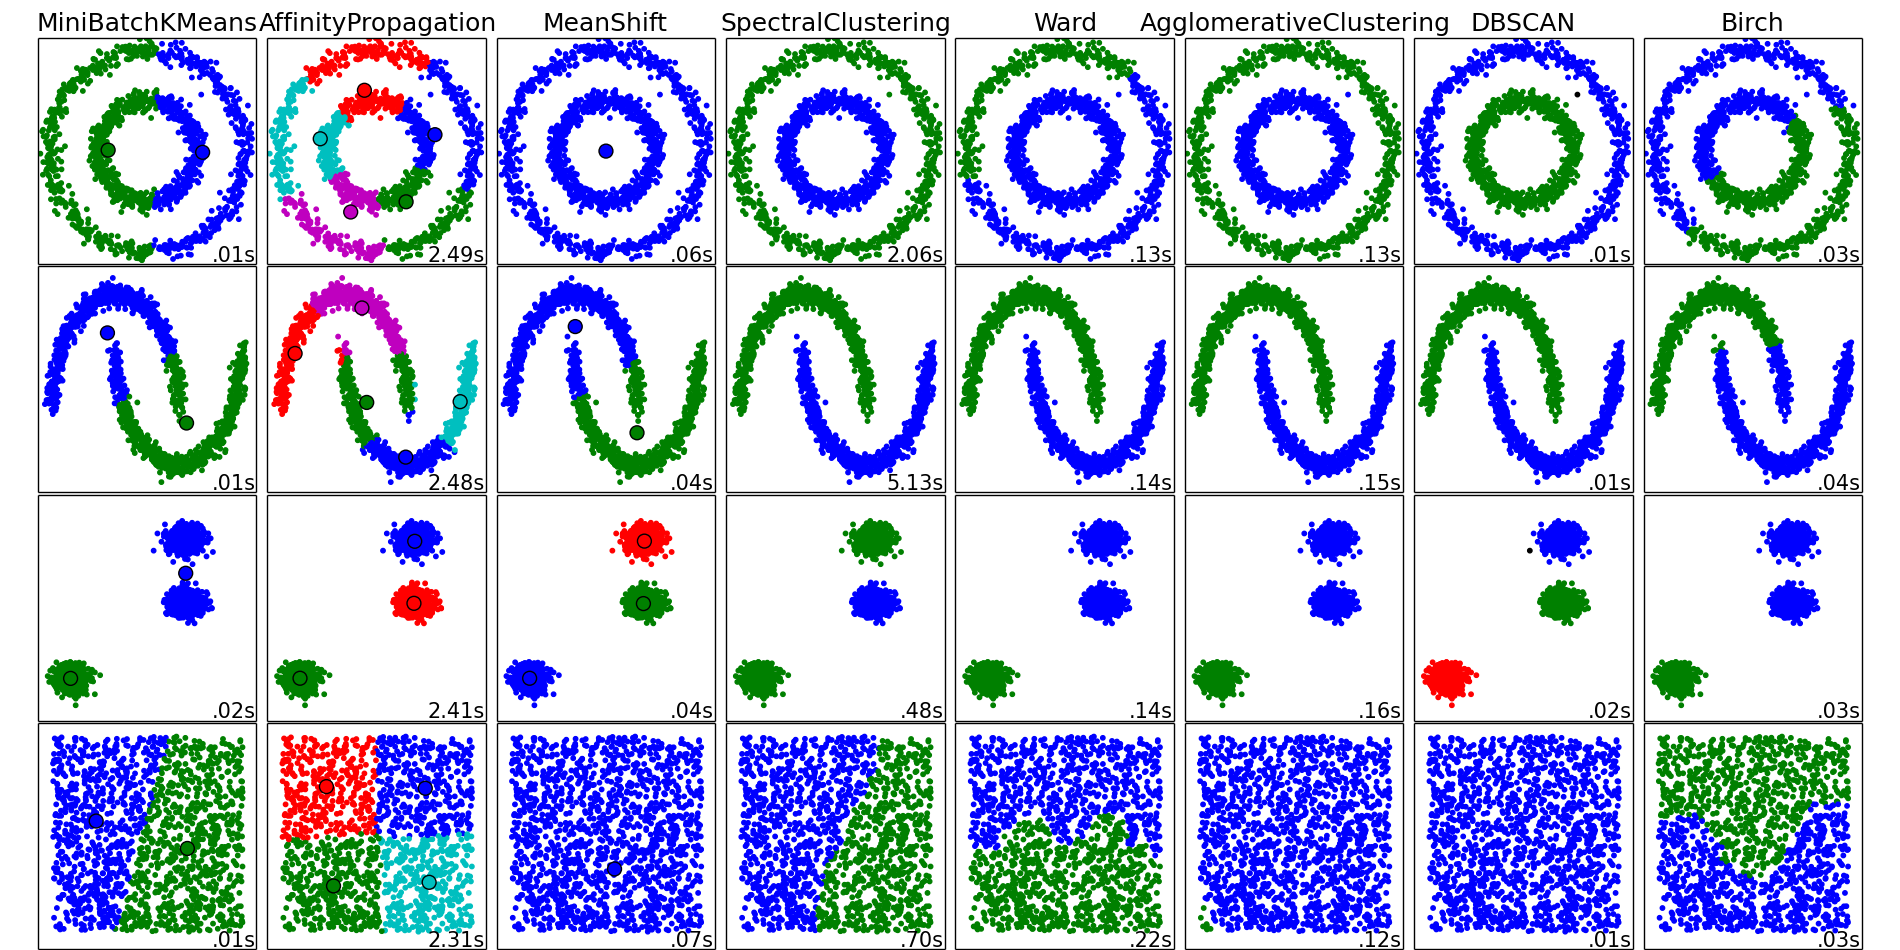
\includegraphics[width=1\linewidth]{figs/plot_cluster_comparison_001.png}
	\end{figure}
	
Taken from \url{http://scikit-learn.org/stable/modules/clustering.html}
	
\end{frame}


\begin{frame}
	\frametitle{Scikit Learn implementations} 

\begin{block}{We will study the following algorithms included in the Scikit-learn module:}
\begin{itemize}
\item K-means
\item Spectral clustering
\item Agglomerative clustering
\end{itemize}
\end{block}

\begin{block}{We will illustrate the performance of the algorithms with the following data}
\begin{itemize}
\item Synthetic data
\item Digit recognition dataset
%\item Olivetti face recognition dataset
\item Images
\end{itemize}
You could also work with your text documents from the previous session, using the ``topic representation'' of each document.

\end{block}

	
\end{frame}

\section{K-means}
\begin{frame}
\frametitle{K-means (1957)}

$K$-means is a centroid-based method that tries to minimize the following distortion function
$$D = \sum_{k=1}^K \sum_{{\bf x} \in {\cal{G}}_k}\|{\bf x}-{\mu}_k\|_2^2$$

\begin{block}{After initialization of centroids:}
\begin{enumerate}
\item Assign each data point to closest centroid
\item Recalculate centroids positions
\item Go back to 1 until no further changes or max iterations achieved
\end{enumerate}
\end{block}

\end{frame}


\begin{frame}
\frametitle{$K$-means initializations}

$K$-means convergence is guaranteed ... but just to a local minimum of $D$.

\begin{block}{Different initialization possibilities:}
\begin{enumerate}
\item $k$-means$++$: To maximize inter-centroid distance
\item Random among training points
\item User-selected
\end{enumerate}
Typically, different runs are executed, and the best one is kept.
\end{block}

Check out \url{http://scikit-learn.org/stable/modules/generated/sklearn.cluster.KMeans.html} for parameters, attributes, and methods.

\end{frame}


\section{Spectral clustering}
\begin{frame}
\frametitle{Spectral clustering}

The key idea of spectral clustering is to search for groups of connected data. I.e, rather than pursuing convex clusters, spectral clustering allows for arbitrary shape clusters.

\begin{block}{Preliminary steps:}
\begin{enumerate}
\item Calculate distances among each pair of training points
\item Obtain an affinity (i.e., similarity) matrix. In doing so, we can set to zero values below a threshold.
\end{enumerate}
\end{block}

$$A_{i,j} = \exp\left(-\alpha\|{\bf x}_i - {\bf x}_j\|_2^2 \right)$$

\end{frame}

\begin{frame}
\frametitle{Spectral clustering (Graph cutting algorithms)}

We split data into groups, so that links between points in the same group have small values, whereas ``across-groups'' links can be have large weight.

\begin{block}{Main steps:}
\begin{enumerate}
\item Obtain the Laplacian of the Graph ($L = D - A$), or a normalized version (variants)
\item Obtain $K$ leading eigenvectors, and project onto them all training data
\item Form clusters in the new space, using, e.g., $K$-means
\end{enumerate}
\end{block}

	\begin{figure}
		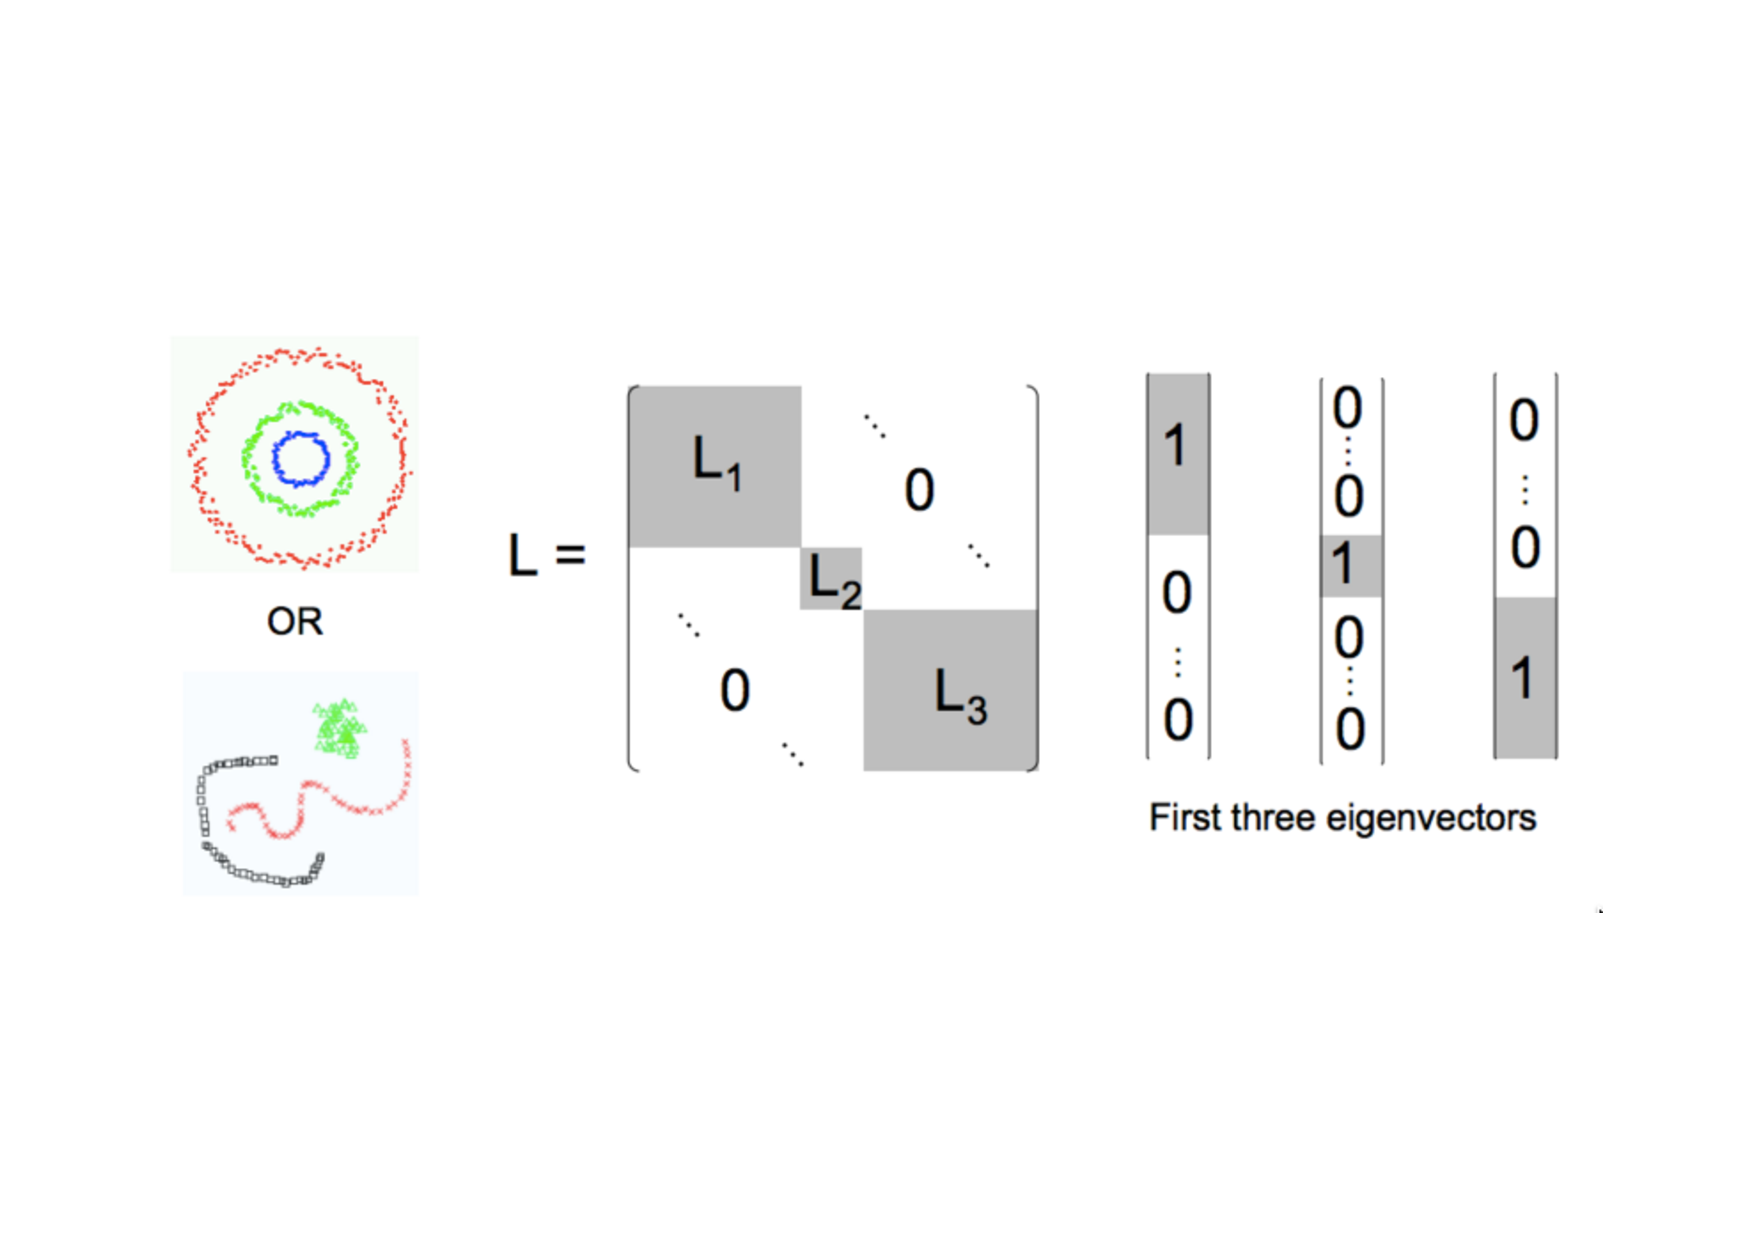
\includegraphics[width=.8\linewidth,clip=true,trim=0 6cm 0 6cm]{figs/spectral_clustering}
	\end{figure}

\vspace{-.4cm}
Taken from \footnotesize{\url{https://charlesmartin14.wordpress.com/2012/10/09/spectral-clustering/}}

\end{frame}



\begin{frame}
\frametitle{Spectral clustering (Graph cutting algorithms)}

The algorithm in Scikit-learn requires the number of clusters to be specified. It works well for a small number of clusters but is not advised when using many clusters and/or data.

\vspace{2cm}

\url{http://scikit-learn.org/stable/modules/generated/sklearn.cluster.SpectralClustering.html}

\end{frame}


\section{Agglomerative Clustering algorithms}
\begin{frame}
\frametitle{Agglomerative/Hierarchical clustering}

\begin{block}{Bottom-up approach:}
\begin{itemize}
\item At the beginning, each data point is a different cluster
\item At each step of the algorithm two clusters are merged, according to certain performance criterion
\item At the end of the algorithm, all points belong to the root node
\end{itemize}
\end{block}

In practice, this creates a hierarchical tree, that can be visualized with a dendogram. We can cut the tree at different levels, in each case obtaining a different number of clusters.
\vspace{-.5cm}
\begin{figure}
		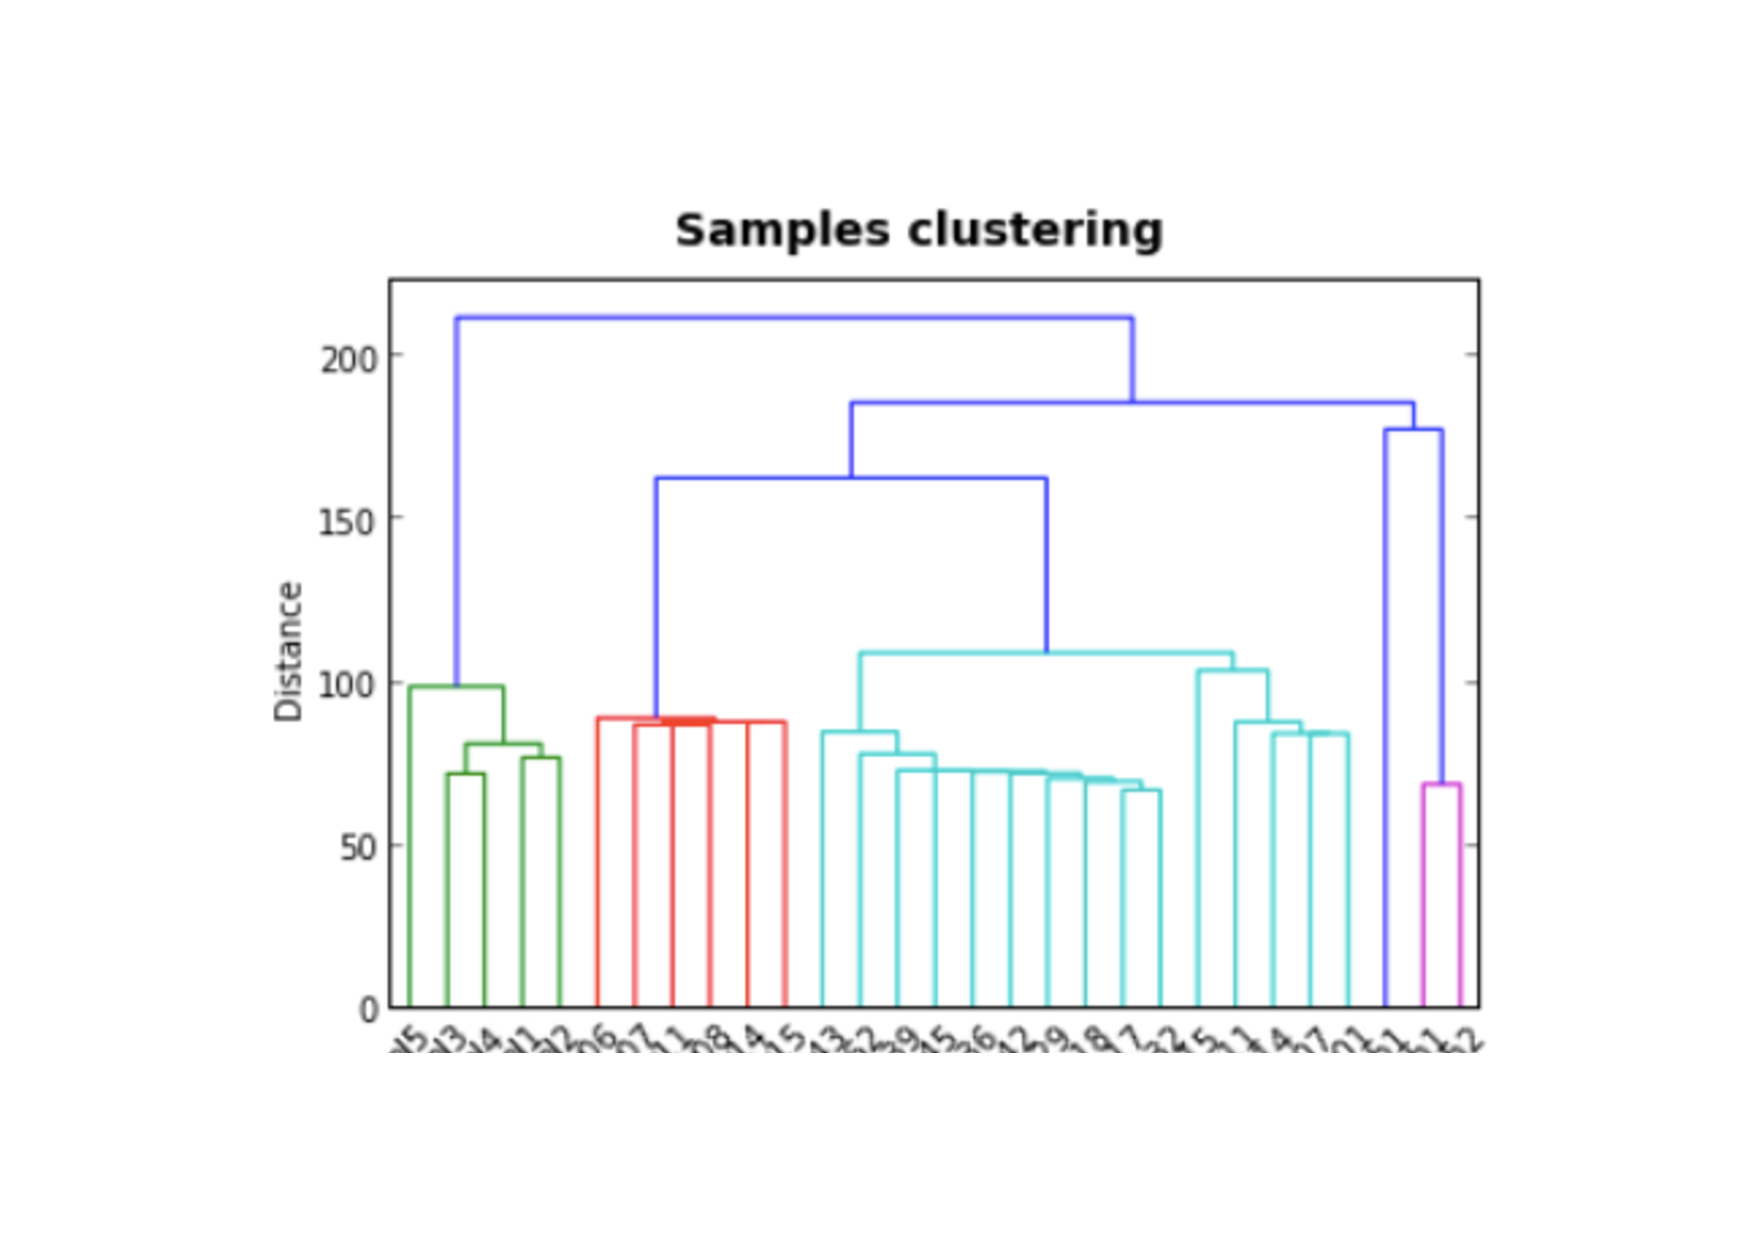
\includegraphics[width=.5\linewidth]{figs/dendogram}
\end{figure}
	
\end{frame}

\begin{frame}
\frametitle{Criteria for merging clusters}

\begin{block}{We merge the two closest clusters, where the distance between clusters is defined as:}
\begin{itemize}
\item Single: Distance between clusters is the minimum of the distances between any two points in the clusters
\item Complete: Maximal distance between any two points in each cluster
\item Average: Average distance between points in both clusters
\item Centroid: Distance between the (Euclidean) centroids of both clusters
\item Ward: We merge centroids so that the overall increment of {\em within-cluster} variance is minimum. 

\end{itemize}
\end{block}

\vspace{-.5cm}
\begin{figure}
		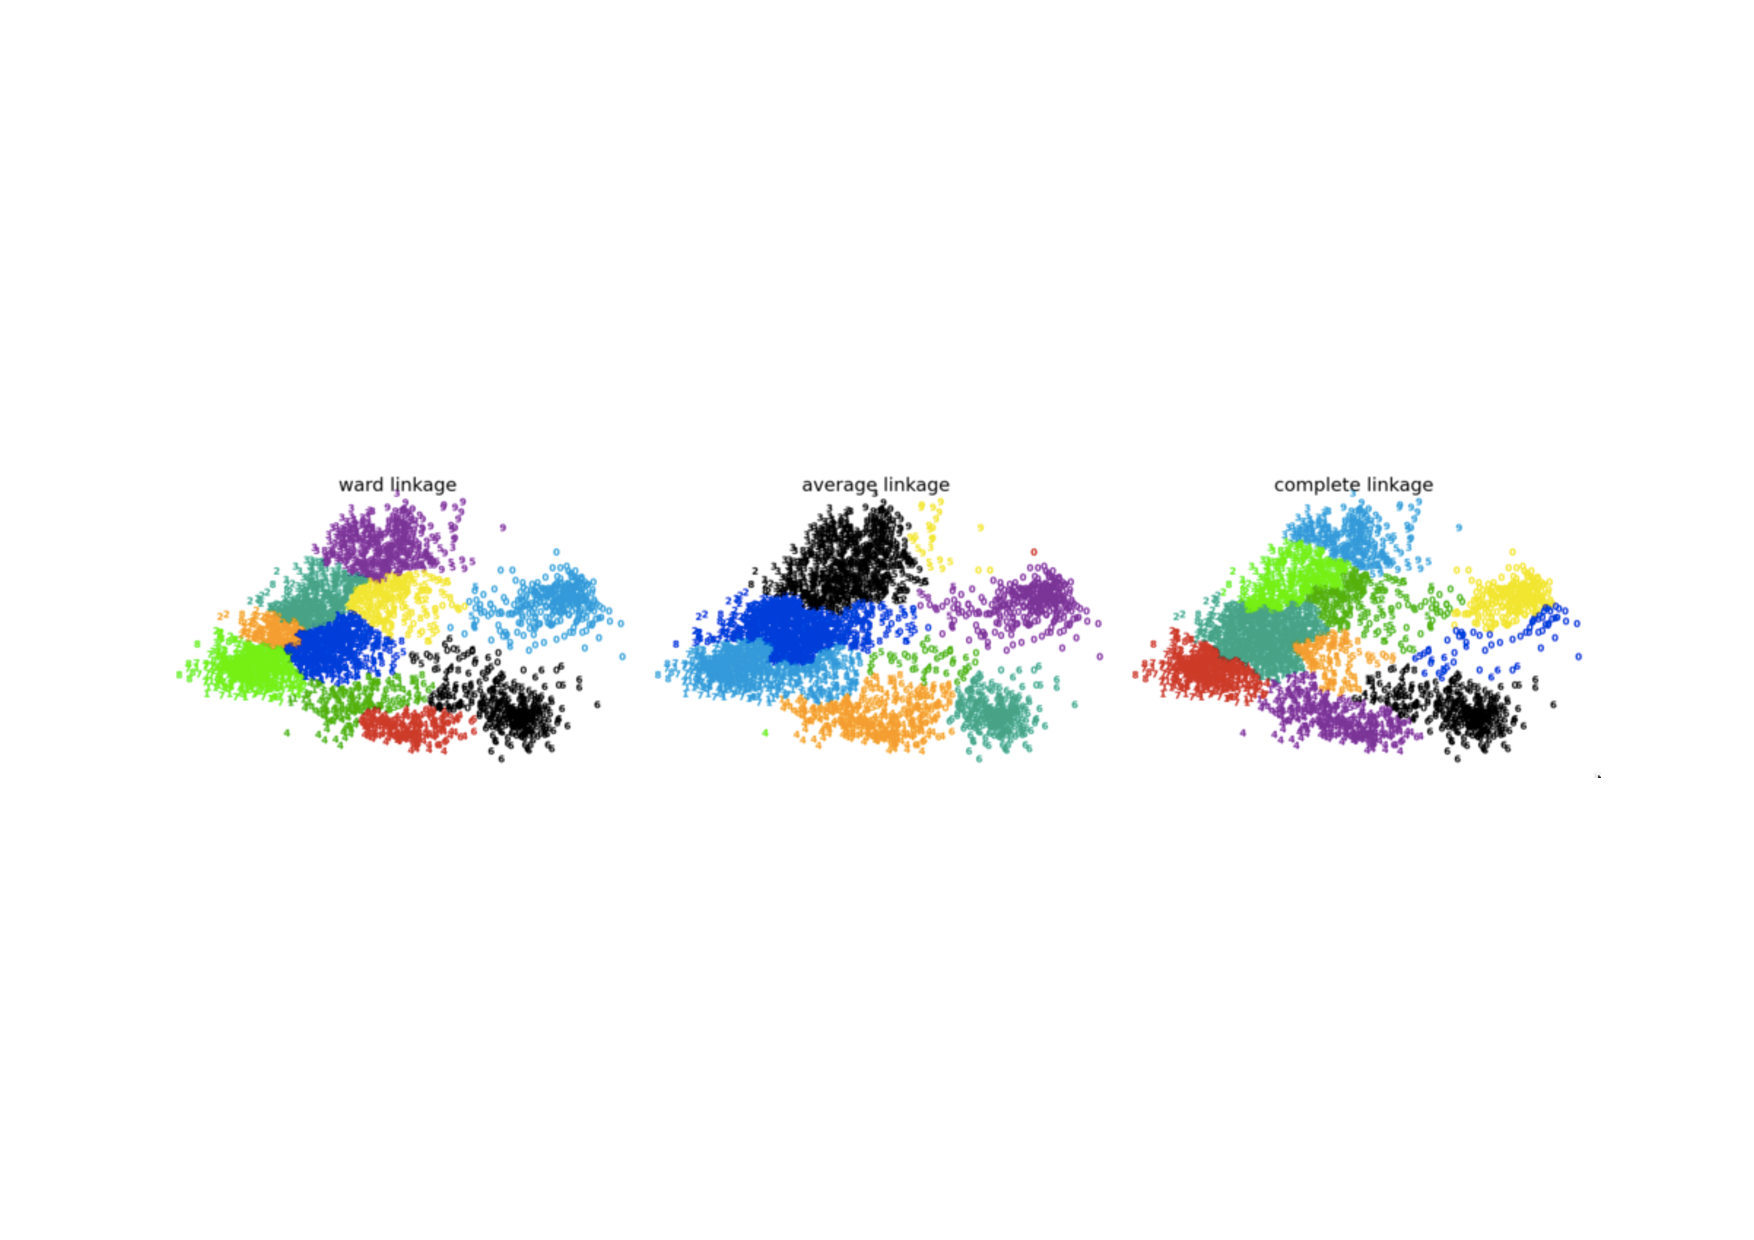
\includegraphics[width=1\linewidth,clip=true,trim=0 7cm 0 7cm]{figs/hcluster_methods}
\end{figure}
	
\end{frame}


\begin{frame}
\frametitle{Python implementations}

Hierarchical clustering may lead to clusters of very different sizes. Complete linkage is the worst strategy, while Ward gives the most regular sizes. However, the affinity (or distance used in clustering) cannot be varied with Ward, thus for non Euclidean metrics, average linkage is a good alternative. 

\vspace{.3cm}

There are at least three different implementations of the algorithm:

\begin{enumerate}

\item Scikit-learn: Only implements `complete', `ward', and `average' linkage methods. Allows for the definition of connectivity constraints
\item Scipy
\item fastcluster: Similar to Scipy, but more efficient with respect to computation and memory.

\end{enumerate}



\end{frame}

%%\begin{frame}
%%\frametitle{Motivation}
%%
%%We are witnessing an explosion of applications where the analysis of data plays a crucial role. As important as data sources are the algorithms to extract the relevant information.
%%
%%\vspace{.5cm}
%%Some application examples:
%%
%%\begin{itemize}
%%
%%\item Internet search engines
%%\item Biomedical applications (automatic classification of patients and diseases)
%%\item Financial Markets forecast / investment
%%\item Recommendation systems 
%%\item ...
%%
%%\end{itemize}
%%
%%\end{frame}
%
%%\begin{frame}
%%\frametitle{Hot topics} 
%%
%%\begin{itemize}
%%\item {\bf Machine Learning}: A field of computer science that deals with algorithms for extracting information from data. 
%%\item {\bf Big Data} (from the wikipedia): Broad term for data sets so large or complex that traditional data processing applications are inadequate. Challenges include analysis, capture, data curation, search, sharing, storage, transfer, visualization, and information privacy.
%%
%%The term often refers simply to the use of predictive analytics or other certain advanced methods to extract value from data, and seldom to a particular size of data set.
%%\item {\bf Internet as Data Source}: An application of big data analysis where the analyzed data is captured from the Internet.
%%\end{itemize}
%%
%%\end{frame}
%
%
%%\begin{frame}
%%	\frametitle{Hot topics} 
%%	
%%	\begin{itemize}
%%		\item {\bf Data Science}: The extraction of knowledge from large volumes of data that are structured (databases) or unstructured (emails, social media, user-generated content).
%%	\end{itemize}
%%	
%%\begin{figure}
%%	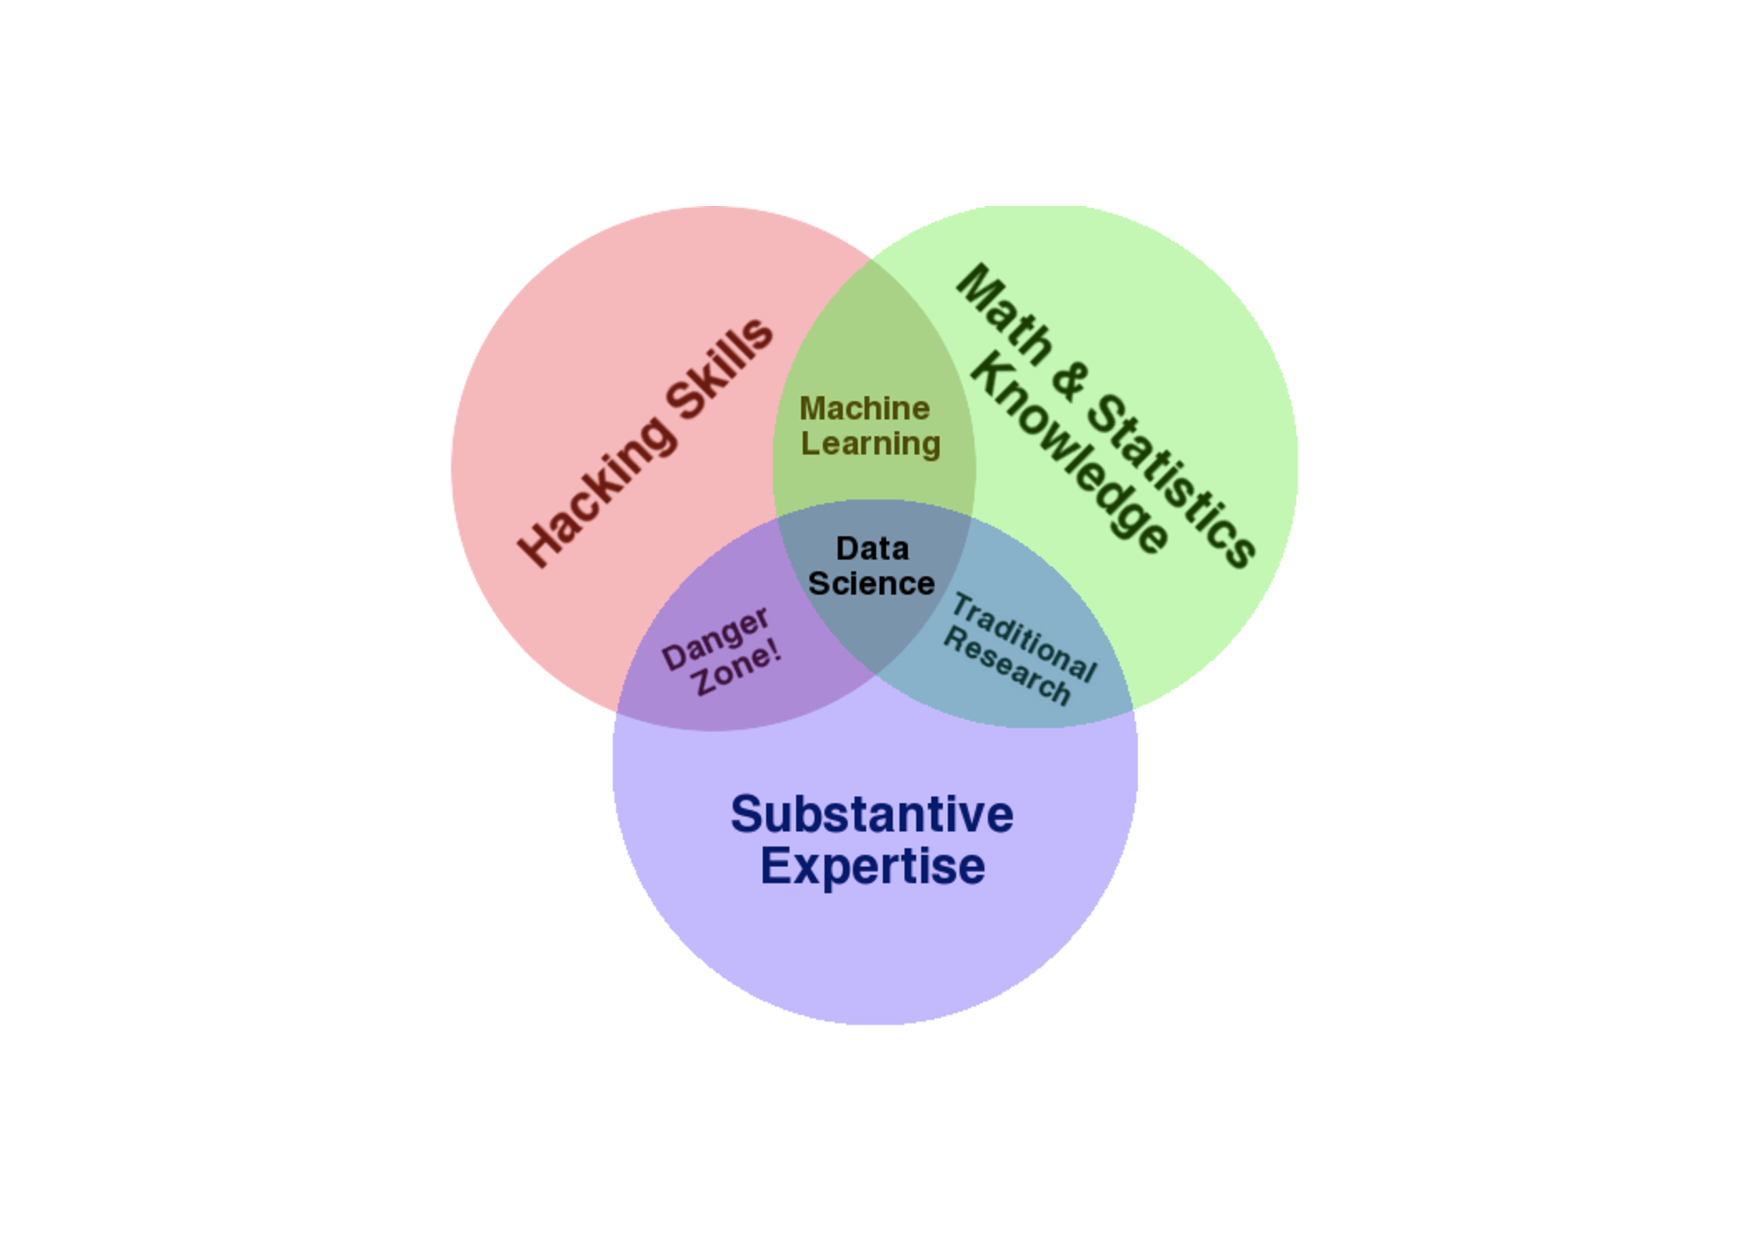
\includegraphics[width=0.6\linewidth,clip=true,trim=3cm 3cm 3cm 3cm]{figs/data_science2}
%%\end{figure}
%%	
%%If you are (really) smart, you can make your life as a data scientist working from home: \url{https://www.kaggle.com/competitions}
%%	
%%\end{frame}
%
%
%
%
%\begin{frame}
%	\frametitle{Organization of the session} 
%
%\Large
%\begin{enumerate}
%%\item Python introduction ($\sim$ 30 min)
%\item Topic modeling presentation ($\sim$ 20 min)
%\item Data download from Arxiv.org ($\sim$ 35 min)
%\item Corpus preprocessing ($\sim$ 35 min)
%\item Topic modeling experiments ($\sim$ 30 min)	
%\end{enumerate}
%	
%	
%\end{frame}
%
%
%%\begin{frame}
%%	\frametitle{1. Python introduction (10'10 to 10'40)} 
%%
%%\begin{columns}[c]	
%%	\column{.65\textwidth} % Left column and width
%%	\begin{enumerate}
%%		\item Log in into the Ubuntu OS	
%%		\item Open a terminal and set up python:
%%		\begin{itemize}
%%			\item[$>$] pip install --user jsonschema
%%			\item[$>$] pip install --user feedparser
%%			\item[$>$] pip install --user --upgrade ipython
%%		\end{itemize}
%%		\item Download and unzip the file:
%%		\url{http://www.tsc.uc3m.es/~jarenas/best.zip}
%%		\item We are going to work with python notebooks
%%		\begin{itemize}
%%			\item[$>$] ipython notebook
%%		\end{itemize}
%%		\item Open and work with the notebook `Python\_intro'
%%	\end{enumerate}
%%	
%%	\column{.35\textwidth} % Right column and width
%%	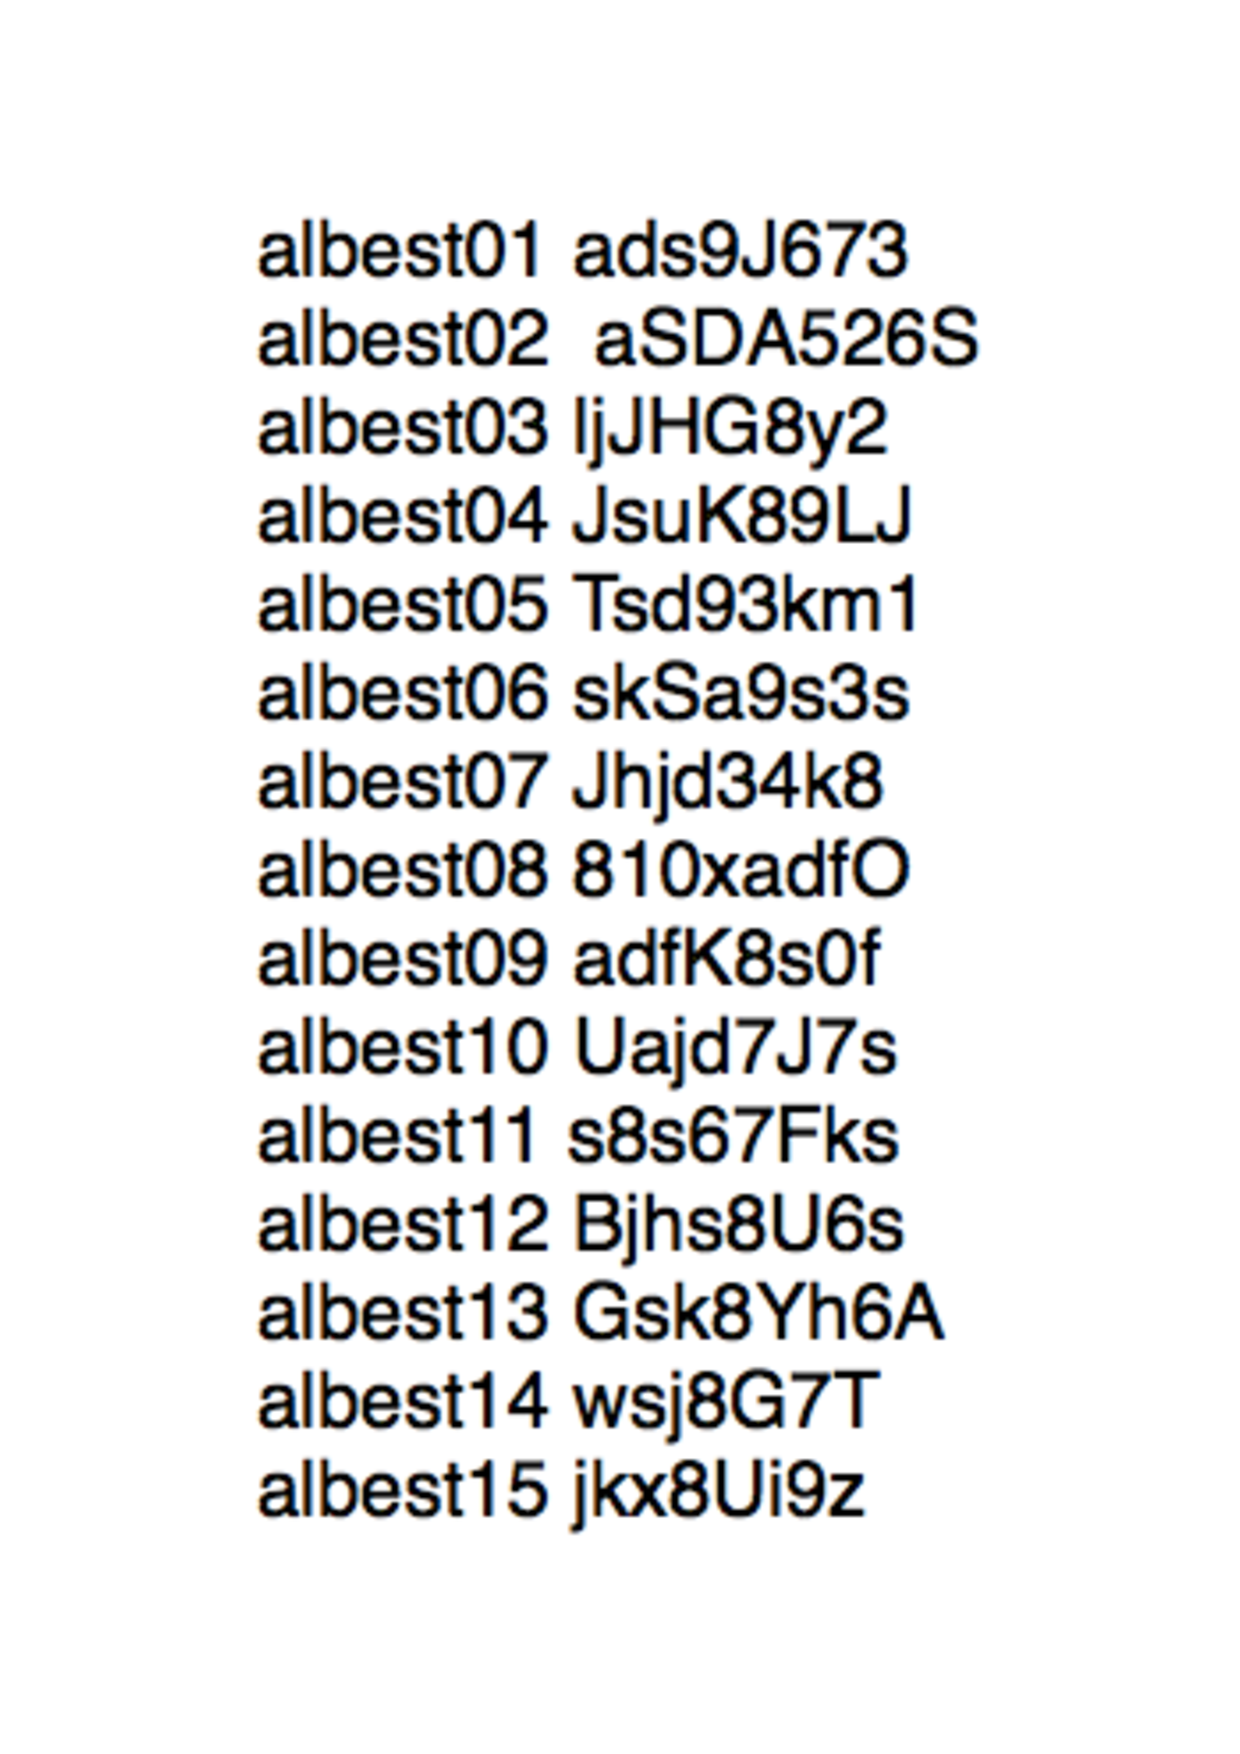
\includegraphics[width=\linewidth,clip=true,trim=3cm 3cm 3cm 2cm]{figs/accounts.pdf}
%%\end{columns}
%%
%%\end{frame}
%
%\begin{frame}
%	\frametitle{1. A brief introduction to topic modeling} 
%	
%Topic Modeling attempts to uncover the underlying semantic structure of a corpus of documents, by identifying recurring patterns of terms.
%\begin{figure}\begin{center}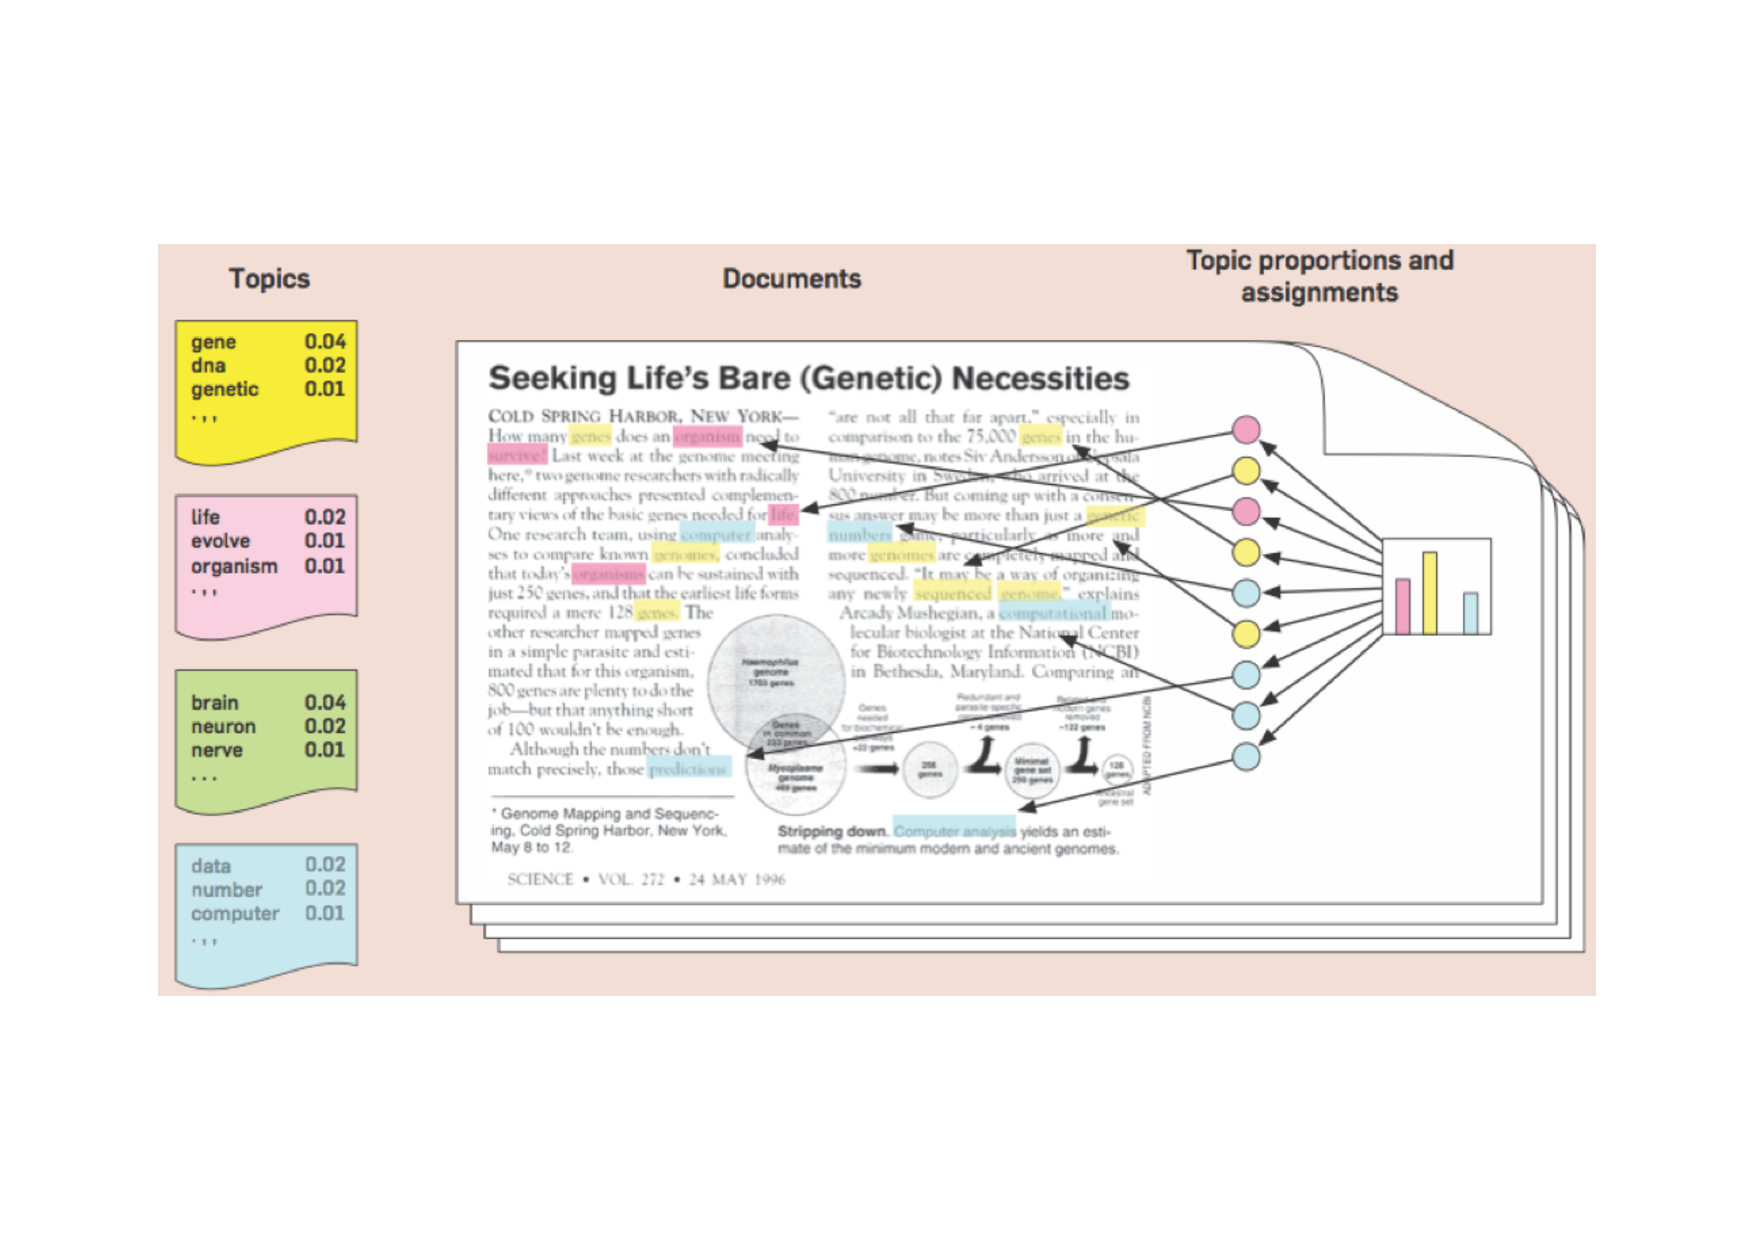
\includegraphics[width=.8\linewidth,clip=true,trim=2cm 3cm 2cm 3cm]{figs/LDA1.pdf}\end{center}\end{figure}
%
%Topic models are useful on their own to build visualizations and explore data. They are also very useful as an intermediate step in many other tasks
%\end{frame}
%
%
%%----------------------------------------------------------------------------------------
%%	PRESENTATION SLIDES
%%----------------------------------------------------------------------------------------
%
%\section[LDA]{Latent Dirichlet Allocation}
%
%\subsection{Basics of LDA}
%
%\begin{frame}
%\frametitle{LDA Generative model}
%\begin{figure}
%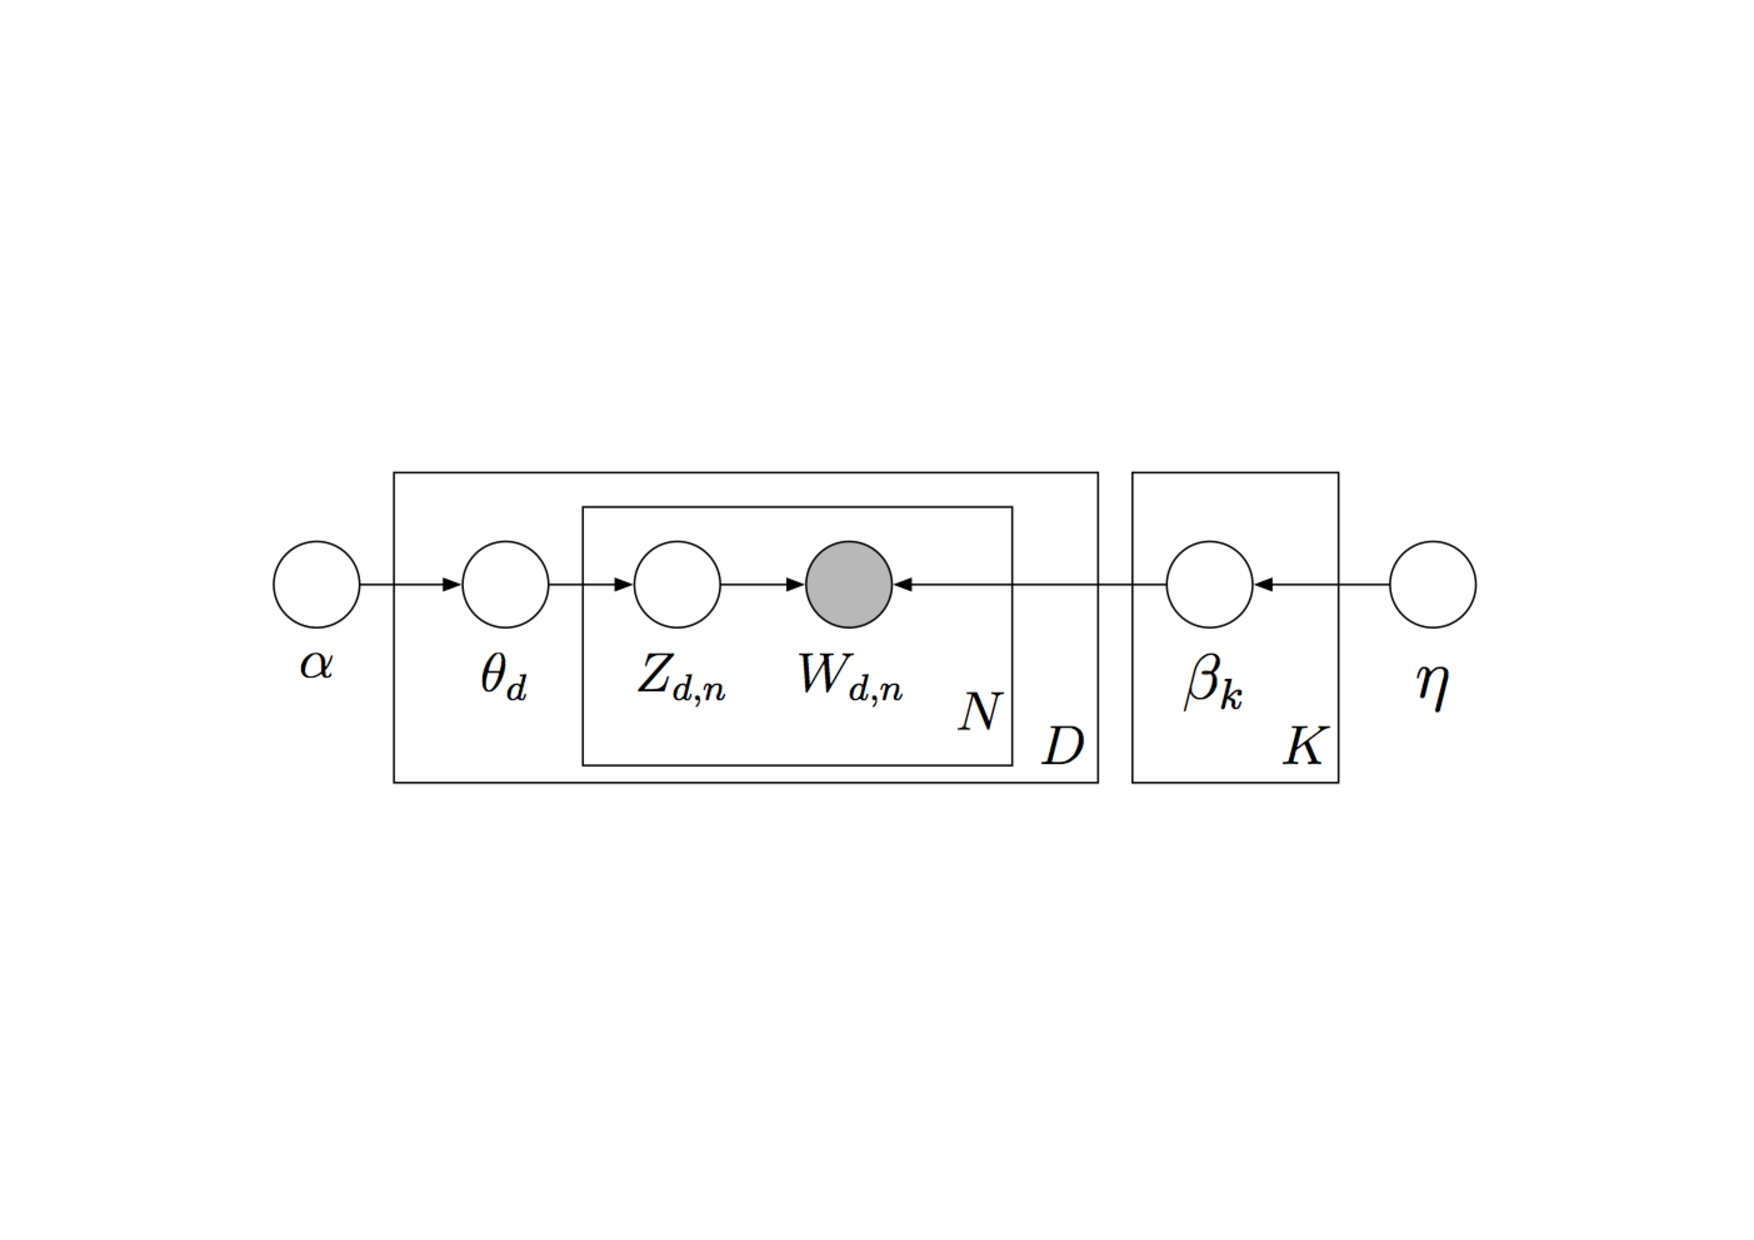
\includegraphics[width=0.8\linewidth,clip=true,trim=3cm 7.5cm 3cm 8cm]{figs/graph_model}
%\end{figure}
%\begin{block}{For each topic}
%\begin{enumerate}
%\item Draw topic distribution: $\betabf_k \sim \text{Dir}_V (\eta)$
%\end{enumerate}
%\end{block}
%\begin{block}{For each document}
%	\begin{enumerate}
%		\item Draw document composition: $\thetabf_d \sim \text{Dir}_K (\alphabf)$
%		\item For each word in document:
%		\begin{enumerate}
%		\item Draw topic assignment: $z_{d,n} \sim \text{Mult}(\thetabf_d) \qquad (\in\{1,\dots,K\})$
%		\item Draw word: $w_{d,n} \sim \text{Mult}(\betabf_{z_{d,n}}) \qquad\qquad\qquad (\in\{1,\dots,V\})$
%		\end{enumerate}
%	\end{enumerate}
%\end{block}
%
%\end{frame}
%
%\begin{frame}
%	\frametitle{LDA Generative model}
%	\begin{figure}
%		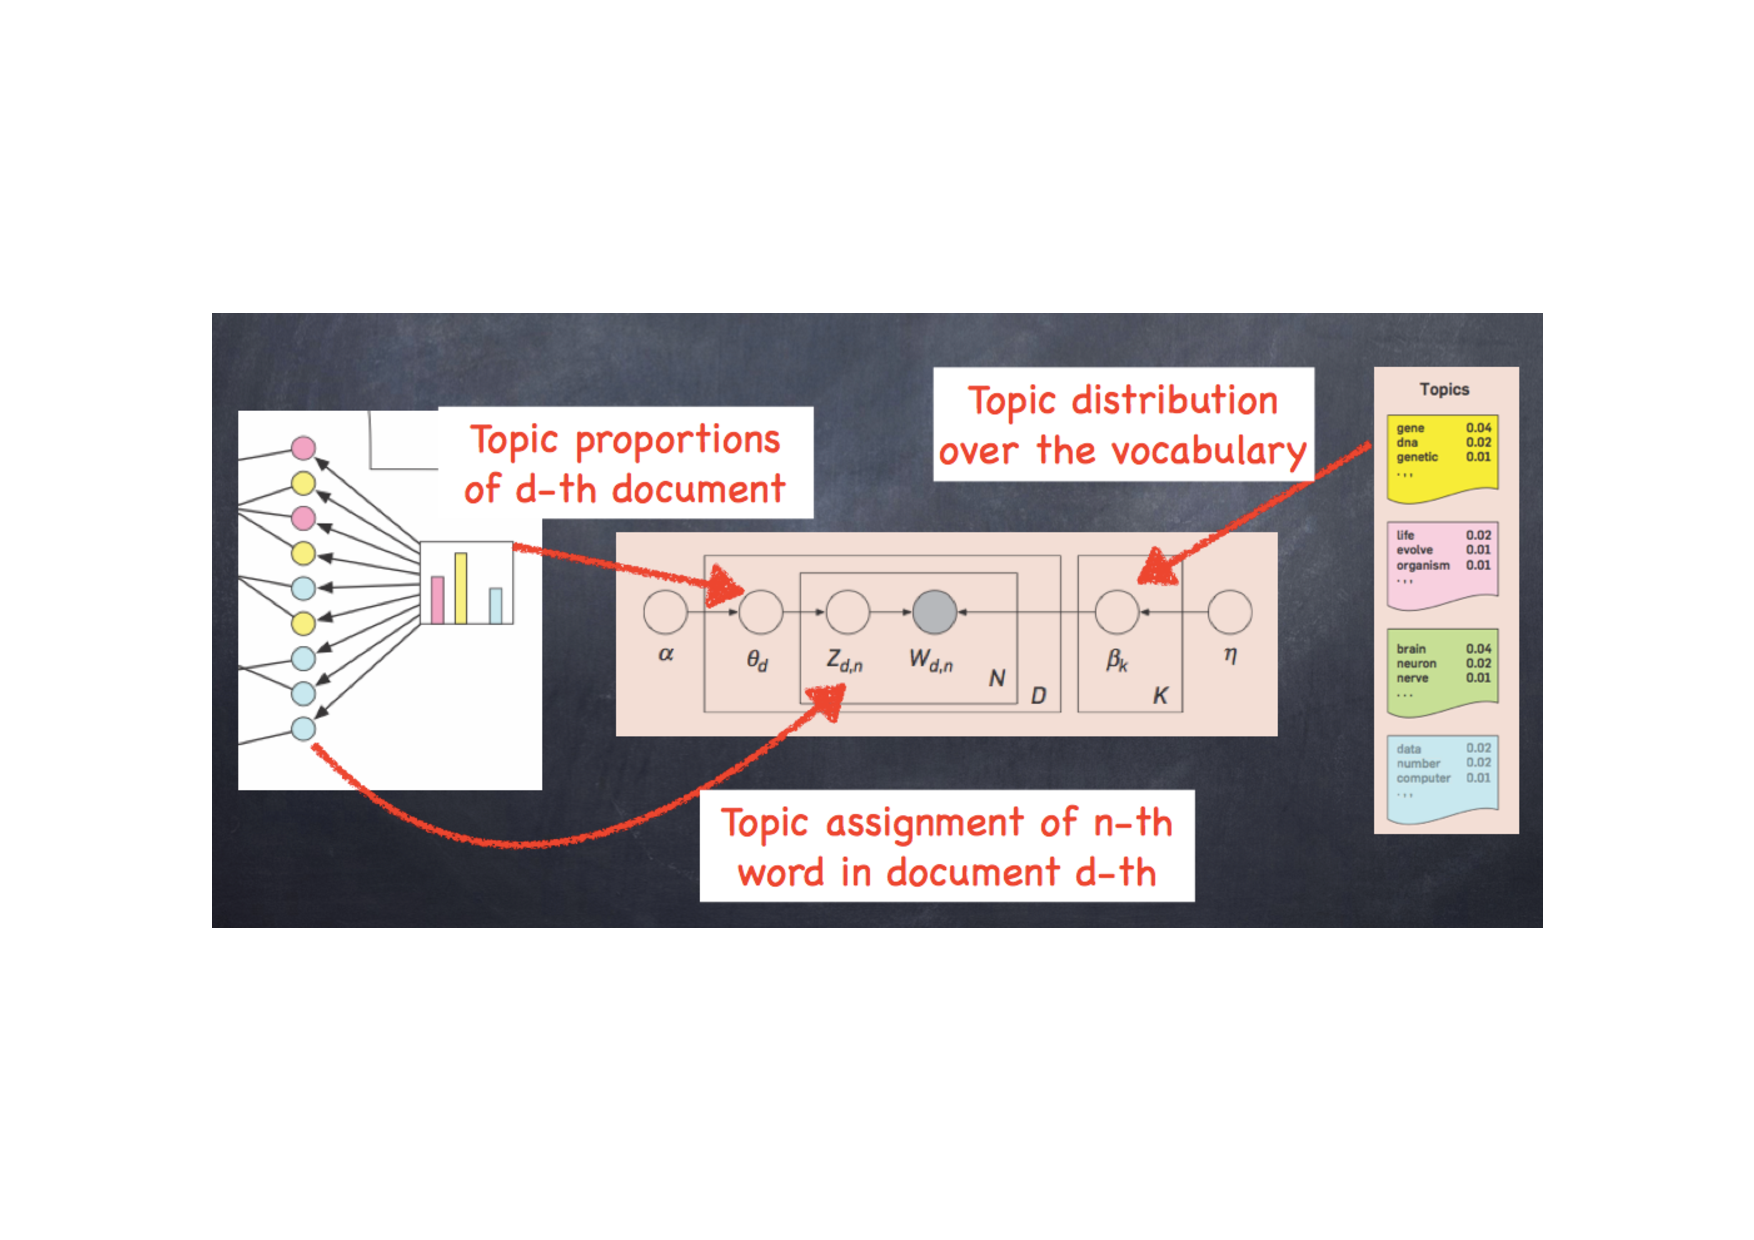
\includegraphics[width=1.1\linewidth,clip=true,trim=3cm 0cm 0cm 3cm]{figs/LDA2}
%	\end{figure}
%	
%\end{frame}
%
%\begin{frame}
%\frametitle{Why Dirichlet?}
%
%\begin{columns}[c] % The "c" option specifies centered vertical alignment while the "t" option is used for top vertical alignment
%	
%	\column{.45\textwidth} % Left column and width
%	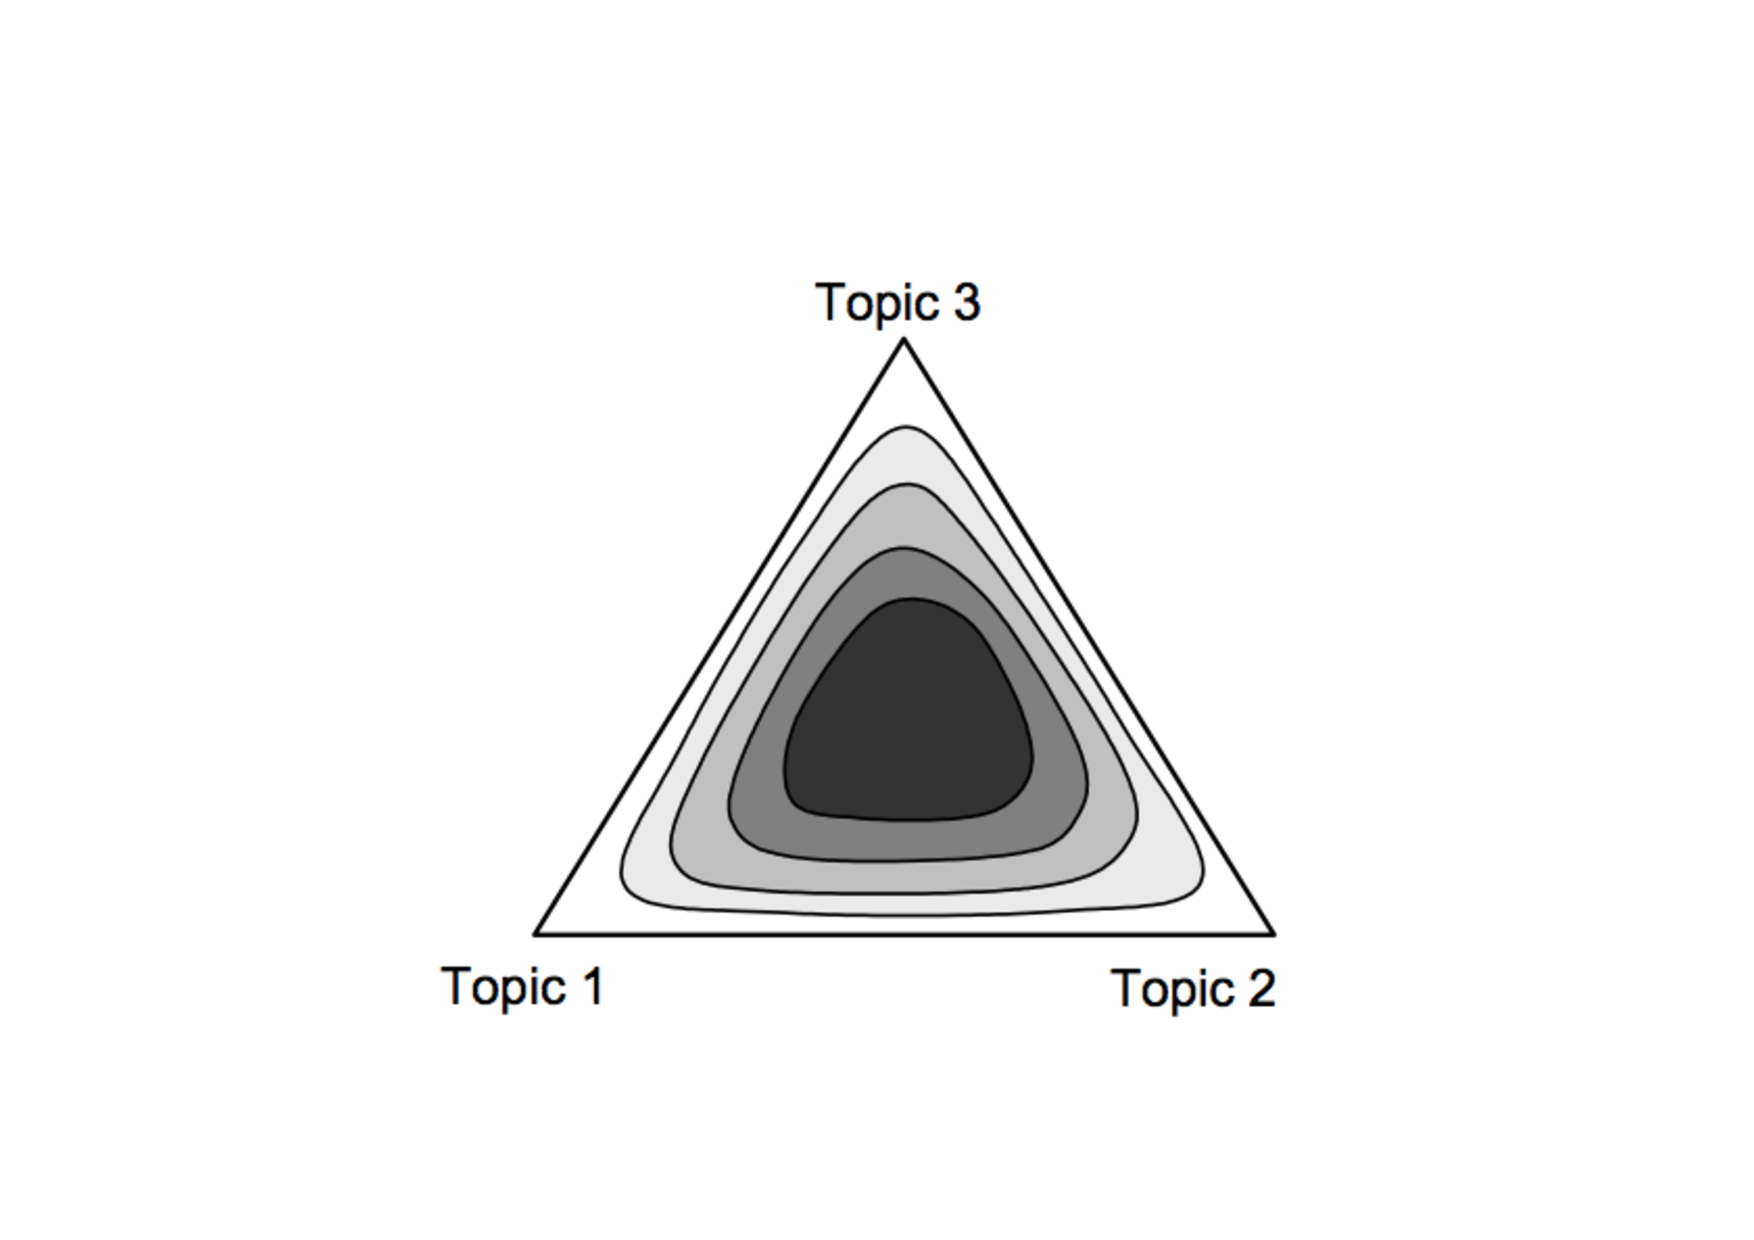
\includegraphics[width=0.8\linewidth,clip=true,trim=7cm 2cm 8cm 2cm]{figs/simplex}
%	
%	$p(\thetabf | \alphabf) = \frac{\Gamma(\sum_k \alpha_k)}{\prod_k \Gamma(\alpha_k)} \prod_k \theta_k^{\alpha_k - 1}$
%
%	\column{.65\textwidth} % Right column and width
%
%	\begin{itemize}
%	\item Extracts samples from the unitary simplex
%	\item Parameter $\alphabf$ controls asymmetry of the distribution, and can be used to favor sparser vectors
%	\item Dirichlet pdf is a conjugated prior of the Multinomial distribution, i.e. 
%	$$\underbrace{p(\thetabf | {\bf z},\alphabf)}_{\text{Dir}} \propto \underbrace{p({\bf z} | \thetabf,\alphabf)}_{\text{Mult}} \underbrace{p(\thetabf | \alphabf)}_\text{Dir}$$
%	\end{itemize}
%	
%\end{columns}
%	
%\end{frame}
%
%
%
%\begin{frame}
%\frametitle{Notation summary}
%
%\begin{table}[c]
%	\small
%\begin{tabular}{l l}
%	\toprule
%	Model constants & \\
%	\midrule
%	Number of Topics & $K$ \\
%	Number of docs & $D$ \\
%	Vocabulary size & $V$ \\
%	Words in each document & $N_d$ \\
%	\midrule
%	Hidden variables (latents) & \\
%	\midrule
%	Topic characterization & $\betabf = \{\betabf_1,\dots,\betabf_K\}$ \\
%	Documents composition & $\thetabf= \{\thetabf_1,\dots,\thetabf_D\}$ \\
%	Token assignments & ${\mathbf Z} = \{z_{d,n}\},\; d=1,\dots,D, \; n=1,\dots,N_d$ \\
%	\midrule
%	Observations & \\
%	\midrule
%	Words & ${\mathbf W} = \{w_{d,n}\},\; d=1,\dots,D, \; n=1,\dots,N_d$ \\
%	\midrule
%	Hyperparameters & \\
%	\midrule
%	Dirichlet parameters & $\alphabf, \eta$ \\
%	\bottomrule
%\end{tabular}
%\end{table}
%
%\end{frame}
%
%
%\begin{frame}
%\frametitle{Information of interest}
%\begin{block}{Joint distribution}
%From the graphic model we can directly read the joint distribution of hidden variables and observations:
%\begin{align}
%p(\thetabf,\betabf&,{\mathbf Z},{\mathbf W}|\alphabf,\eta) = p(\betabf | \eta) p(\thetabf|\alphabf) p({\mathbf Z} | \thetabf) p({\mathbf W} | \betabf {\mathbf Z}) \nonumber \\
%& = \nonumber� \prod_{k=1}^K p(\betabf_k |� \eta) \prod_{d=1}^D p(\thetabf_d | \alphabf) \prod_{n=1}^{N_d} p(z_{d,n}� | \thetabf_d) p(w_{d,n} | \betabf_{z_{d,n}})
%\end{align}
%\end{block}
%
%\begin{block}{Exploring the corpus}
%\begin{itemize}
%\item Documents composition: $\widehat{\thetabf} = \mathbb{E}\{\thetabf | {\mathbf W}\}$
%\item Exploring the topics: $\widehat{\betabf} = \mathbb{E}\{\betabf | {\mathbf W}\}$
%\item Detailed study of docs: $\widehat{\mathbf Z} = \mathbb{E}\{{\mathbf Z} | {\mathbf W}\}$
%\end{itemize}
%\end{block}
%
%\end{frame}
%
%
%
%\begin{frame}
%	\frametitle{Some popular LDA implementations}
%		\begin{itemize}
%			\item Mallet (Java): \url{http://mallet.cs.umass.edu/topics.php}
%			\item Gensim (Python):
%			\url{https://radimrehurek.com/gensim/}
%			\item Blei's group (C):
%			\url{https://www.cs.princeton.edu/~blei/lda-c/index.html}
%		\end{itemize}
%	
%\end{frame}
%
%\begin{frame}
%	\frametitle{2. Data download \\ 3. Corpus preprocessing} 
%	
%		\begin{enumerate}
%			\item Open and work with the notebook `create\_arxiv\_corpus'
%		\end{enumerate}
%		
%
%\end{frame}
%
%
%\begin{frame}
%	\frametitle{4. Topic modeling of corpuses}
%	\begin{block}{Topic extraction}
%	\begin{enumerate}
%		\item Download source code from
%		\url{https://www.cs.princeton.edu/~blei/lda-c/index.html}
%		\item From the terminal, cd into folder 'lda-c-dist', and compile the code:
%		\begin{itemize}
%			\item[$>$] make
%		\end{itemize}
%		\item Now, you can extract topics using a command like
%		\begin{itemize}
%			\item[$>$] lda est [initial alpha] [k] [settings] [data] [random/seeded/*] [directory]
%		\end{itemize}
%		Read the readme.txt file or ask the teachers to get more information about the meaning of each of these input parameters
%		
%	\end{enumerate}
%	\end{block}
%	
%	\begin{block}{Topic visualization}
%		\begin{enumerate}
%			\item Use the provided python script 'visualize\_topics.py':
%			\begin{itemize}
%				\item[$>$] python visualize\_topics.py
%			\end{itemize}
%			\item If you have any time left, ask your teacher for assistance about graphic visualizations with D3.
%		\end{enumerate}
%	\end{block}
%	
%\end{frame}

%%%\begin{frame}
%%%\frametitle{Variational Bayes implementation}
%%%\begin{enumerate}
%%%\item We try to infer the posterior of the hidden variables:
%%%$$p(\thetabf,\betabf,{\mathbf Z}|{\mathbf W},\alphabf,\eta) = \frac{p(\thetabf,\betabf,{\mathbf Z},{\mathbf W}|\alphabf,\eta)}{p({\mathbf W}|\alphabf, \eta)} $$
%%%This distribution is intractable, due to impossibility to integrate out all latent variables in the denominator.
%%%\item Variational Bayes approximation:
%%%$$p(\thetabf,\betabf,{\mathbf Z}|{\mathbf W},\alphabf,\eta) \approx q(\thetabf,\betabf,{\mathbf Z}) = q_\theta(\thetabf|{\mathbf W}) q_\beta(\betabf|{\mathbf W}) p({\mathbf Z}|\thetabf,\betabf,{\mathbf W})$$
%%%\item Solve the following problem:
%%%$$\arg \min D_{KL}(p(\thetabf,\betabf,{\mathbf Z}|{\mathbf W},\alphabf,\eta) \| q(\thetabf,\betabf,{\mathbf Z}))$$
%%%\end{enumerate}
%%%
%%%\end{frame}
%%%
%%%\begin{frame}
%%%	\frametitle{Variational Bayes implementation: Solution}
%%%\begin{block}{Approximate posteriors}
%%%	\begin{itemize}
%%%	\item $\betabf_k \sim \text{Dir}_V(\lambdabf_k)$
%%%	\item $\thetabf_d \sim \text{Dir}_K(\gammabf_d)$
%%%	\end{itemize}
%%%\end{block}		
%%%
%%%\begin{itemize}
%%%\item Deriving closed-form solutions for updating $\lambdabf_k$ and $\gammabf_d$ is rather involved.
%%%\item Equations are coupled, so we need to iterate. The algorithm is guaranteed to converge (to a local minimum).
%%%\item On the solution, $q_\theta(\thetabf)$ and $q_\beta(\betabf)$ approximate the marginal distributions of these variables. This implies that $\lambdabf_k$ and $\gammabf_d$ provide (after normalization) the required expectations $\widehat{\betabf}_k$ and $\widehat{\thetabf}_d$.
%%%\end{itemize}
%%%\end{frame}
%%%
%%%\begin{frame}
%%%\frametitle{Collapsed Gibbs sampling implementation}
%%%
%%%\begin{itemize}
%%%\item Integrating out $\thetabf$ and $\betabf$ in the joint distribution is doable, so we can obtain a closed-form solution for
%%%$$p({\mathbf W},{\mathbf Z} | \alphabf, \eta)$$
%%%\item As discussed before, it is not possible to integrate out $\mathbf Z$, so we cannot obtain the posterior of ${\mathbf Z}$ analytically.
%%%\item Gibbs sampling can be used to approximate such posterior.
%%%\item ``Collapsed'' because we have integrated out $\thetabf$ and $\betabf$.
%%%\end{itemize}
%%%\begin{block}{Properties of the Gibbs method}
%%%\begin{itemize}
%%%\item Analytical expressions are easier to derive
%%% than for VB.
%%%\item We sample the true posterior. However, accuracy is not necessarily better than VB given the sampling.
%%%\item Normally converges slower than the VB solution.
%%%\end{itemize}
%%%\end{block}
%%%
%%%\end{frame}
%%%
%%%\section[Gibbs]{Review of Gibbs Sampling}
%%%
%%%\begin{frame}
%%%\frametitle{Review of Gibbs sampling method}
%%%\begin{block}{Objective}
%%%Obtain samples from the joint distribution $p(z_1,\dots,z_n)$
%%%\end{block}
%%%
%%%\begin{block}{Algorithm}
%%%\begin{enumerate}
%%%\item Start with some initial value: ${\mathbf z}^{(0)} = \{z_1^{(0)},\dots,z_n^{(0)}\}$
%%%\item To get the next sample ${\bf z}^{(i+1)}$ we draw a new value for each variable from the conditional distribution
%%%\begin{align}p(z_j | z_1^{(i+1)},&\dots,z_{j-1}^{(i+1)},z_{j+1}^{(i)},\dots,z_n^{(i)}) \nonumber \\ & \propto p(z_1^{(i+1)},\dots,z_{j-1}^{(i+1)},z_j,z_{j+1}^{(i)},\dots,z_n^{(i)}) \nonumber
%%%\end{align}
%%%\item Iterate until reaching the desired number of samples.
%%%\end{enumerate}
%%%\end{block}
%%%
%%%\end{frame}
%%%
%%%\begin{frame}
%%%	\frametitle{Properties of Gibbs sampling method}
%%%		\begin{itemize}
%%%			\item After a {\it burn-in} period, samples $\{{\mathbf z}^{(i)} \}$ approximate the joint distribution.
%%%			\item If we pick a subset of variables from each sample, we can approximate the marginal pdf of the selected samples.
%%%			\item We can use samples to estimate statistic information of the joint distribution, but:
%%%			\begin{itemize}
%%%				\item First samples should be discarded
%%%				\item We should pick only one every $m$ samples (due to correlation among close samples)
%%%			\end{itemize}
%%%			\item Typically, several chains are run in parallel to prevent the algorithm to become trapped in an island of probability.
%%%		\end{itemize}
%%%	
%%%	
%%%\end{frame}
%%%
%%%\section[LDA Gibbs]{LDA solution based on collapsed Gibbs sampling}
%%%
%%%\begin{frame}
%%%\frametitle{LDA inference with Gibbs sampling}
%%%
%%%\begin{itemize}
%%%\item Each sample consists of the assignments of all words in the corpus: $N = \sum_{d=1}^D N_d$.
%%%\item Integrating out $\thetabf$ and $\betabf$, and after some more or less tedious manipulation:
%%%$$P(z_{d,n}=k, \bar{\mathbf Z}, {\mathbf W}|\alphabf, \eta)\propto \frac{\bar n_d^k + \alpha_k}{\sum_{k'} \bar n_d^{k'} + \alpha_{k'}} \frac{\bar n_{w_{d,n}}^k + \eta}{\sum_{r=1}^V \bar n_r^{k} + \eta}$$
%%%where
%%%	\begin{itemize}
%%%		\item $\bar{\mathbf Z} = {\mathbf Z} - \{z_{d,n}\}$ 
%%%		\item $\bar n_d^k$: Number of words in doc $d$ that have been assigned to topic $k$ (ignoring current assignment of $z_{d,n}$).
%%%		\item $\bar n_r^k $: Number of times that word $r$ has been assigned to topic $k$ (ignoring current assignment of $z_{d,n}$).
%%%	\end{itemize}
%%%\end{itemize}
%%%
%%%\end{frame}
%%%
%%%
%%%\begin{frame}
%%%\frametitle{Intuition}
%%%
%%%\begin{itemize}
%%%	\item $\frac{\bar n_d^k + \alpha_k}{\sum_{k'} \bar n_d^{k'} + \alpha_{k'}}$ is an estimation of $\widehat{\theta}_d^k = \mathbb{E}\{\theta_d^k\}$ excluding $z_{d,n}$.
%%%	\item $\frac{\bar n_{w_{d,n}}^k + \eta}{\sum_{r=1}^V \bar n_r^{k} + \eta}$ is an estimation of $\widehat{\beta}_k^{w_{d,n}} = \mathbb{E}\{\beta_k^{w_{d,n}}\}$ excluding $z_{d,n}$.
%%%		
%%%\end{itemize}
%%%
%%%\vspace{.5cm}
%%%These expressions show that smaller $\alpha_k$ and $\eta$ will favor sparser documents topic composition, and sparser topic descriptions.
%%%
%%%\end{frame}
%%%
%%%
%%%\begin{frame}
%%%\frametitle{Collapsed Gibbs Sampling for LDA: Implementation}
%%%	
%%%\begin{block}{Initialization}
%%%\begin{enumerate}
%%%\item Initialize ${\bf Z}^{(0)}$ as a vector of length $N$ and random components from $\{1,\dots,K\}$.
%%%\item Compute matrices with counts of ocurrences:
%%%\begin{itemize}
%%%	\item ${\mathbf N}_D$: Size ($D\times K$); each position $n_d^k$ contains the number of tokens assigned to topic $k$ in document $d$. 
%%%	\item ${\mathbf N}_W$: Size ($K \times V$); each position $n_r^k$ contains the number of ocurrences of word $r$ that are assigned to topic $k$.
%%%\end{itemize}
%%%\end{enumerate}
%%%\end{block}	
%%%
%%%\end{frame}
%%%
%%%\begin{frame}
%%%	\frametitle{Collapsed Gibbs Sampling for LDA: Implementation}
%%%
%%%\begin{block}{Gibbs sampling (for $l=1,2, \dots$)}
%%%	\begin{enumerate}
%%%		\item For each token $z_{d,n}$ with current assignment $k'$ and associated word $w_{d,n} = r'$:
%%%		\begin{itemize}
%%%			\item Decrement by 1 corresponding positions of ${\mathbf N}_D$ and ${\mathbf N}_W$.
%%%			\item Compute $P(z_{d,n}=k, \bar{\mathbf Z}, {\mathbf W}|\alphabf, \eta)\propto \frac{(\bar n_d^k + \alpha_k)(\bar n_{w_{d,n}}^k + \eta)}{\sum_{r=1}^V \bar n_r^{k} + \eta}$
%%%			\item Draw new topic assignment for $z_{d,n}$ from a multinomial with previous parameters.
%%%			\item Increment by 1 corresponding positions of ${\mathbf N}_D$ and ${\mathbf N}_W$.
%%%		\end{itemize}
%%%		\item Save current sample ${\mathbf z}^{(l)}$
%%%		\item Iterate until desired number of samples is obtained.
%%%	\end{enumerate}
%%%\end{block}	
%%%
%%%\end{frame}
%%%
%%%
%%%\begin{frame}
%%%	\frametitle{Collapsed Gibbs Sampling for LDA: Implementation}
%%%	
%%%	\begin{block}{Outputs}
%%%			\begin{itemize}
%%%				\item ${\widehat{\thetabf}}_d$ can be obtained by summing $\alphabf$ the $d$th row of ${\mathbf N}_D$, and renormalizing the result.
%%%				\item ${\widehat{\betabf}}_k$ can be obtained by summing $\eta$ the $k$th row of ${\mathbf N}_W$, and renormalizing the result.
%%%			\end{itemize}
%%%	\end{block}	
%%%	
%%%	
%%%	\begin{block}{Sample averaging}
%%%		\begin{itemize}
%%%			\item It is typical to average samples, both from different chains and from the same chain.
%%%			\item In Gibbs LDA we should skip this, because there is no guarantee that topics will have the same order in different samples.
%%%			\item We can use samples from same or different chains to assess the stability of topics.
%%%		\end{itemize}
%%%	\end{block}	
%%%
%%%
%%%\end{frame}
%%%
%%%
%%%\section[LDA Spark]{LDA implementation for spark}
%%%
%%%\begin{frame}
%%%	\frametitle{Parallelizing Gibbs sampling for LDA}
%%%	
%%%	\begin{itemize}
%%%		\item It should be clear that we need to compute each chain in parallel
%%%		\item Distribute sampling among processors, trying to avoid as much as possible conflicts between documents and words
%%%		\item For P processors, we split the dataset into $P \times P$ partitions that are then sequentially processed:
%%%	\end{itemize}
%%%		\begin{figure}
%%%		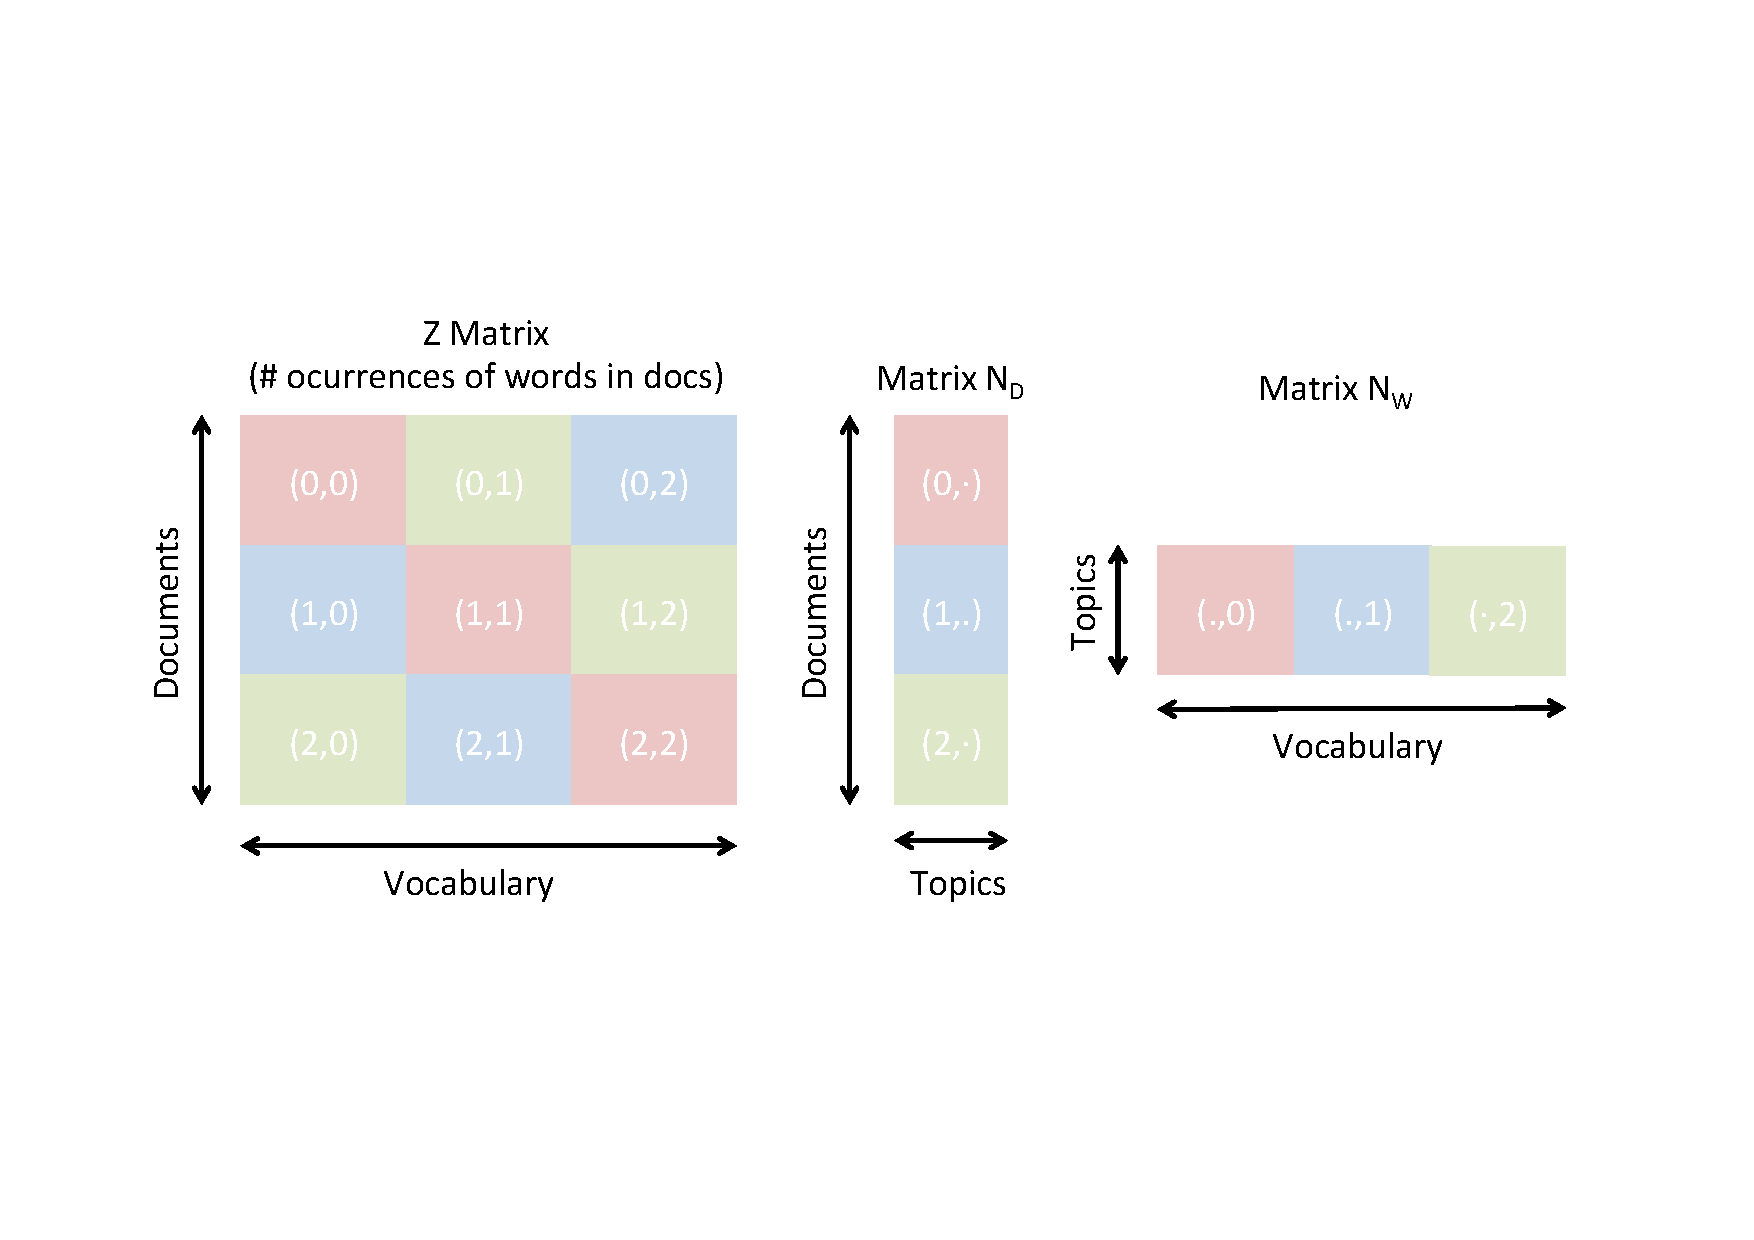
\includegraphics[width=0.8\linewidth,clip=true,trim=2cm 4cm 2cm 4cm]{figs/partitions}
%%%		\end{figure}
%%%\end{frame}
%%%
%%%
%%%
%%%\begin{frame}
%%%	\frametitle{Assigning partitions to processors}
%%%	
%%%	\begin{figure}
%%%		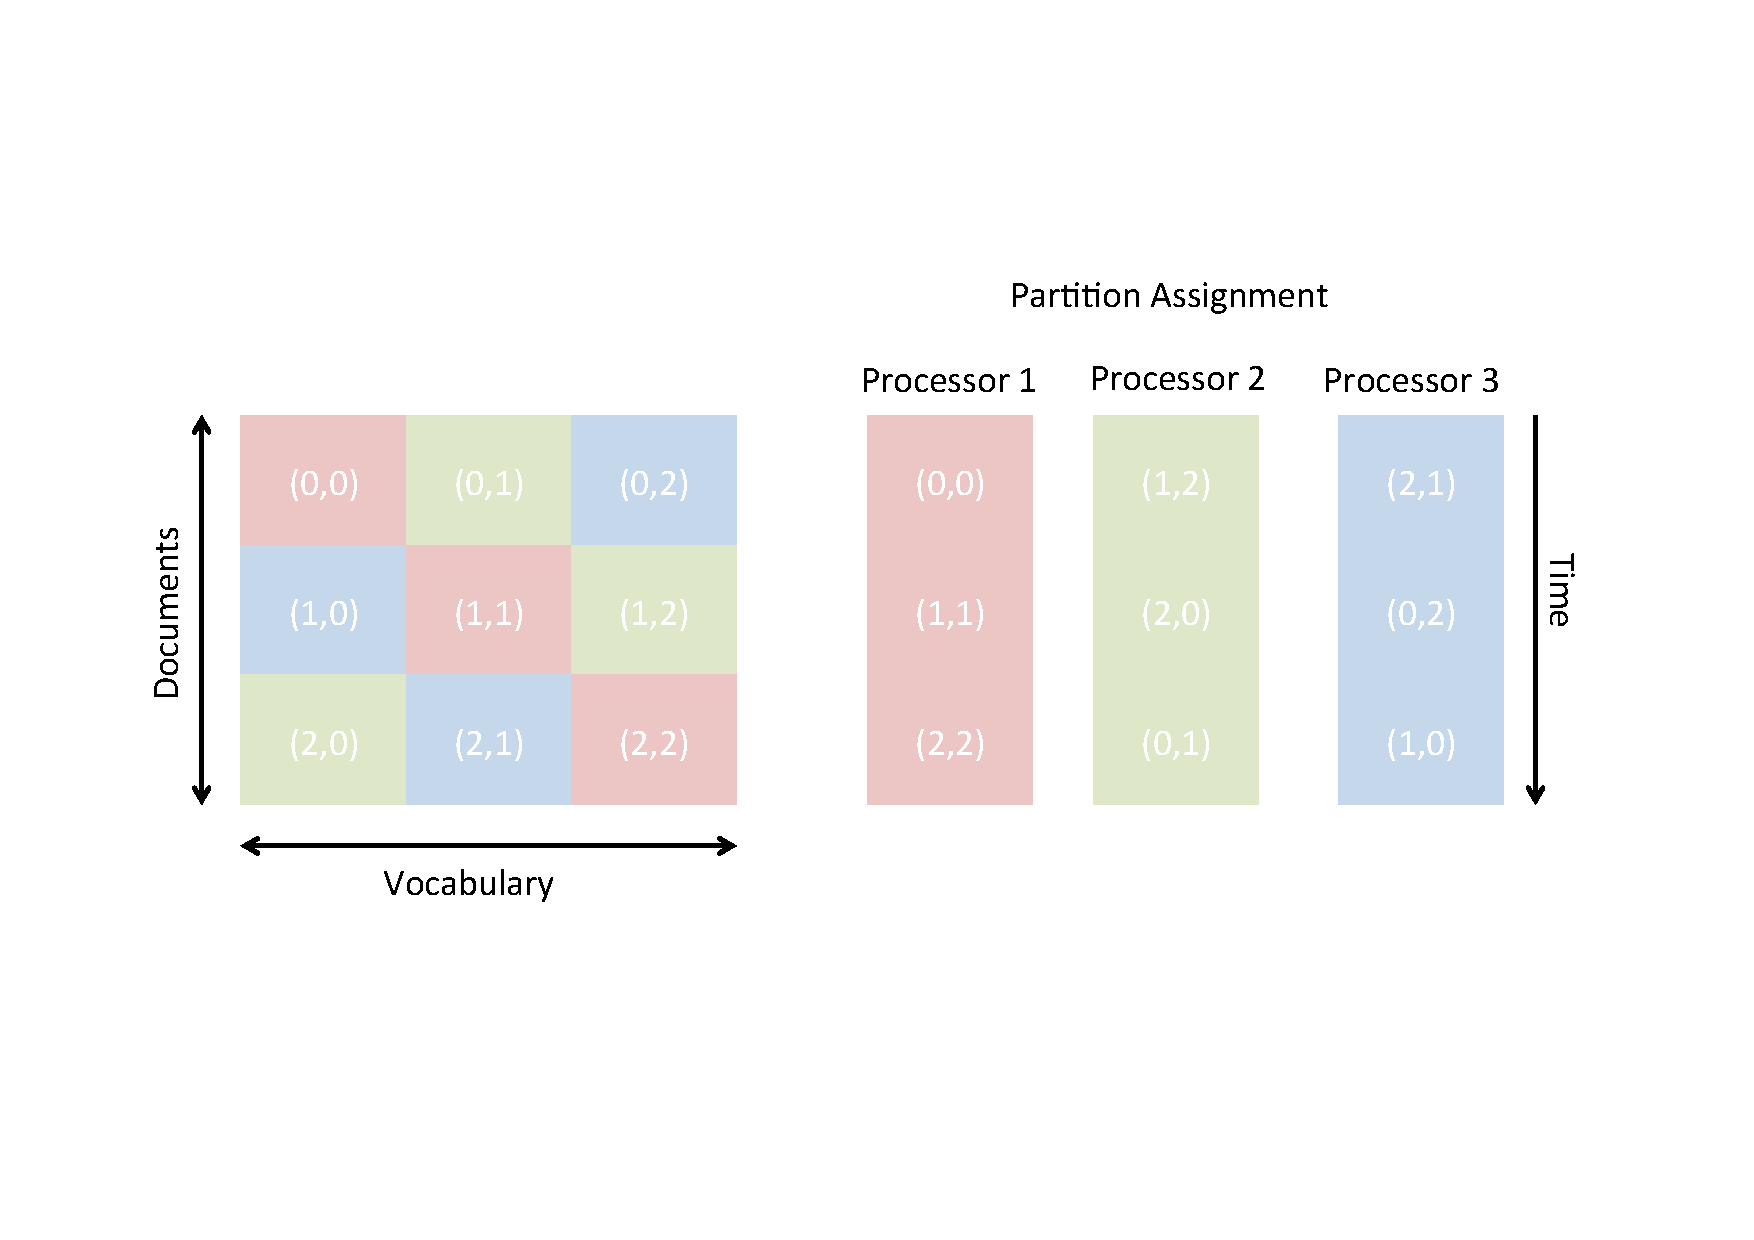
\includegraphics[width=0.8\linewidth,clip=true,trim=2cm 5.3cm 2cm 4.8cm]{figs/assignment}
%%%	\end{figure}
%%%
%%%
%%%	\begin{itemize}
%%%		\item At each time each processor access (and update) different parts of matrices ${\mathbf N}_D$ and ${\mathbf N}_W$
%%%		\item To minimize idle time, ideally all processors should be assigned, at each time, blocks with approximately same number of $z_{d,n}$
%%%		\begin{itemize}
%%%			\item First, split ${\bf Z}$ columnwise, and swap columns until the $P$ partitions have approximately the same number of samples
%%%			\item Split ${\bf Z}$ rowwise, and swap columns randomly, keeping the changes that improve CPU efficiency
%%%		\end{itemize}
%%%	\end{itemize}
%%%	\begin{figure}
%%%		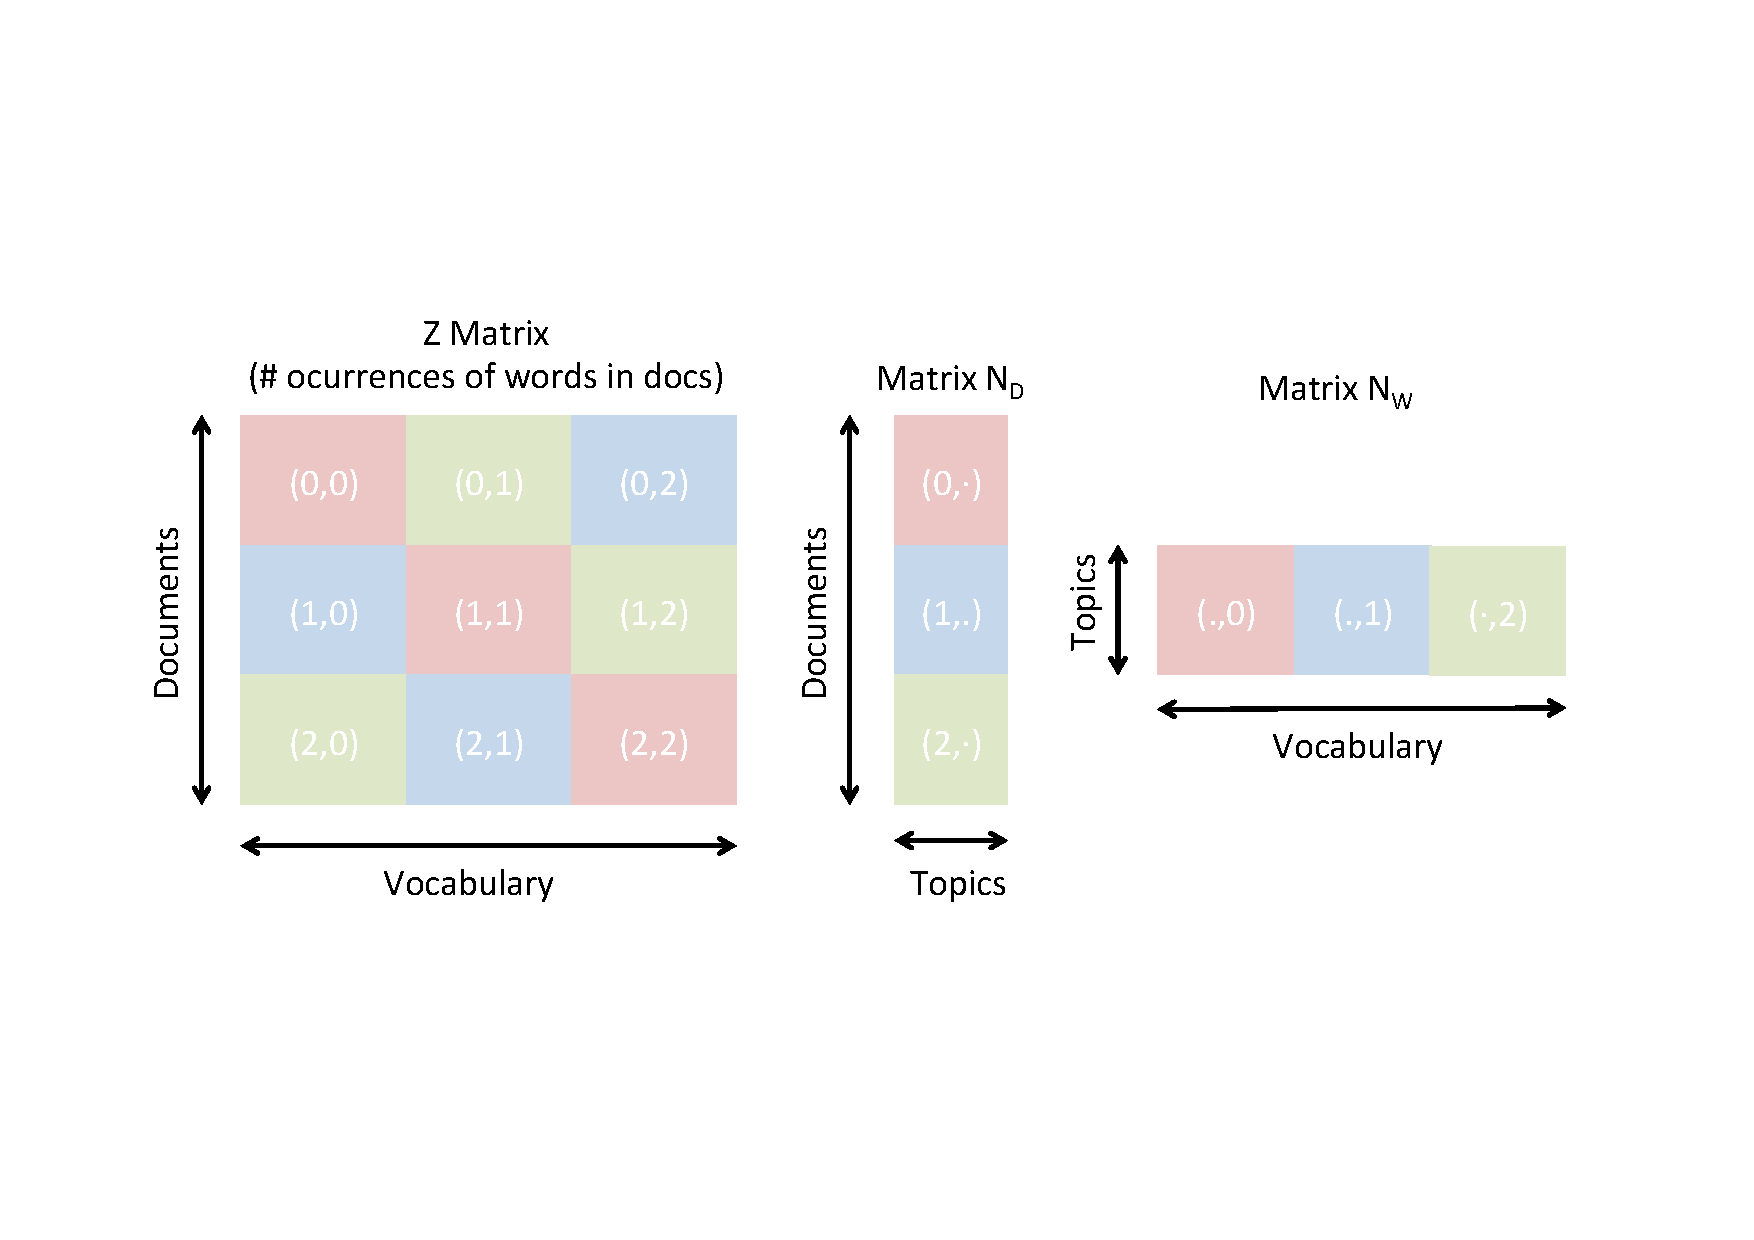
\includegraphics[width=0.8\linewidth,clip=true,trim=2cm 4cm 2cm 4cm]{figs/partitions}
%%%	\end{figure}
%%%\end{frame}
%%%
%%%
%%%\begin{frame}
%%%	\frametitle{Conflicts}
%%%	
%%%	\begin{figure}
%%%		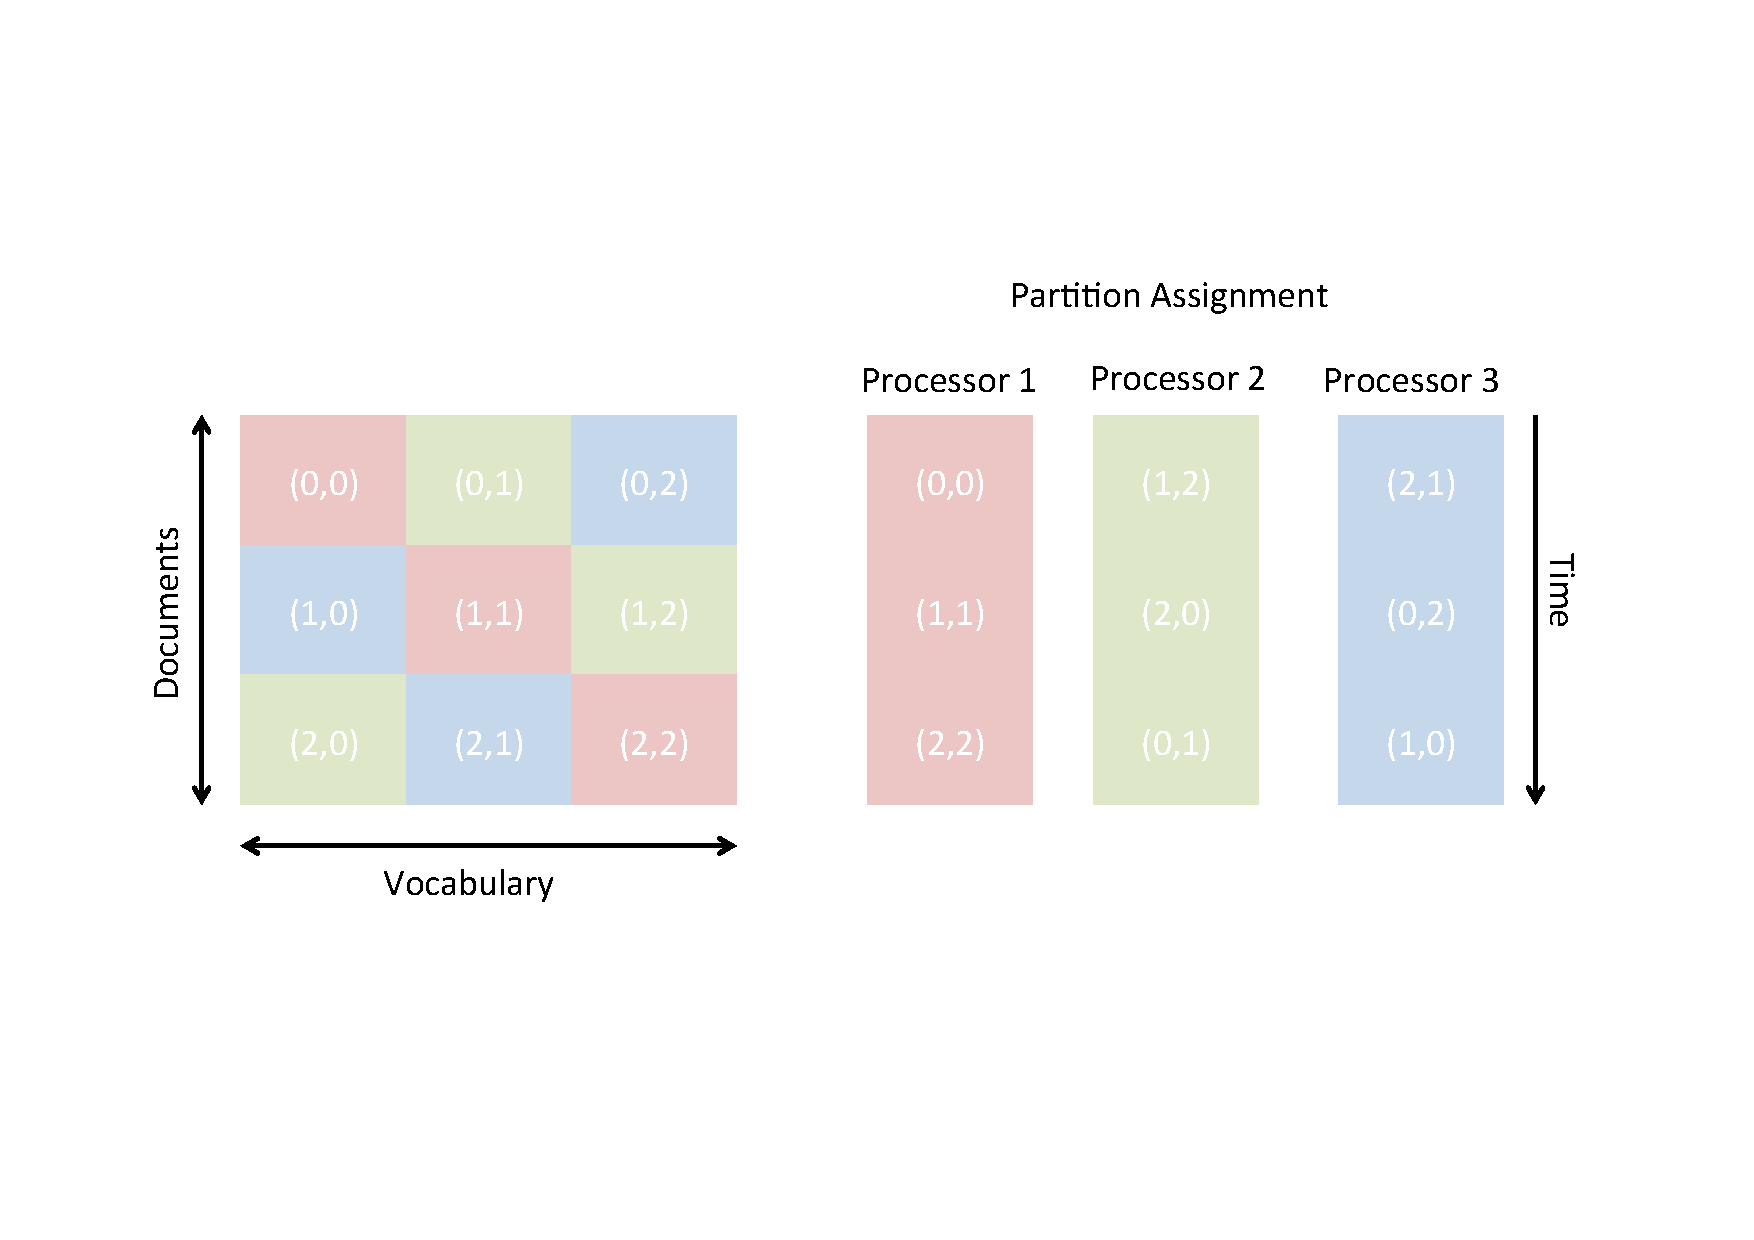
\includegraphics[width=0.8\linewidth,clip=true,trim=2cm 5.3cm 2cm 4.8cm]{figs/assignment}
%%%	\end{figure}
%%%	
%%%	
%%%	\begin{itemize}
%%%		\item At each time each processor access (and update) different parts of matrices ${\mathbf N}_D$ and ${\mathbf N}_W$
%%%		\item To minimize idle time, ideally all processors should be assigned, at each time, blocks with approximately same number of $z_{d,n}$
%%%		\begin{itemize}
%%%			\item First, split ${\bf Z}$ columnwise, and swap columns until the $P$ partitions have approximately the same number of samples
%%%			\item Split ${\bf Z}$ rowwise, and swap columns randomly, keeping the changes that improve CPU efficiency
%%%		\end{itemize}
%%%	\end{itemize}
%%%	\begin{figure}
%%%		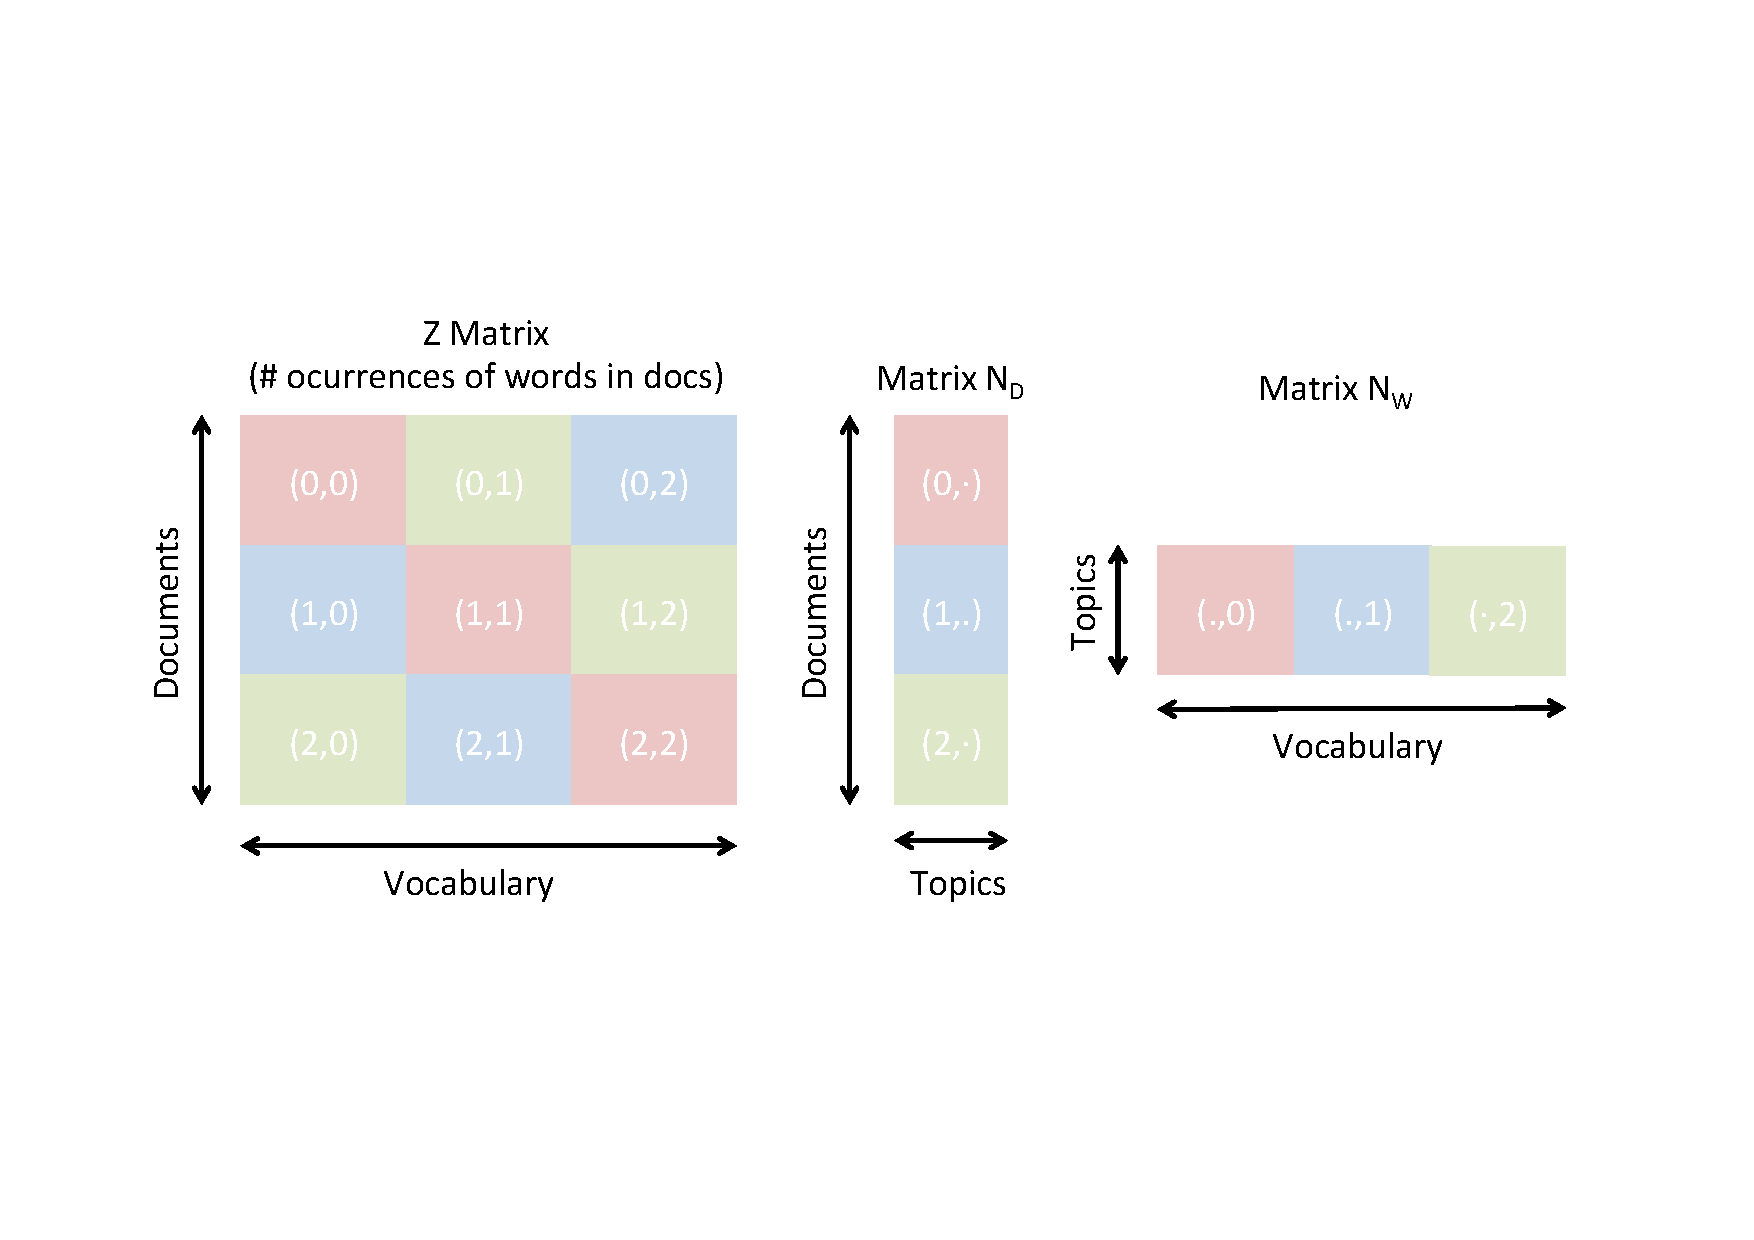
\includegraphics[width=0.8\linewidth,clip=true,trim=2cm 4cm 2cm 4cm]{figs/partitions}
%%%	\end{figure}
%%%\end{frame}
%%%
%%%
%%%
%%%\begin{frame}
%%%	\frametitle{Conflicts}
%%%	
%%%	\begin{figure}
%%%		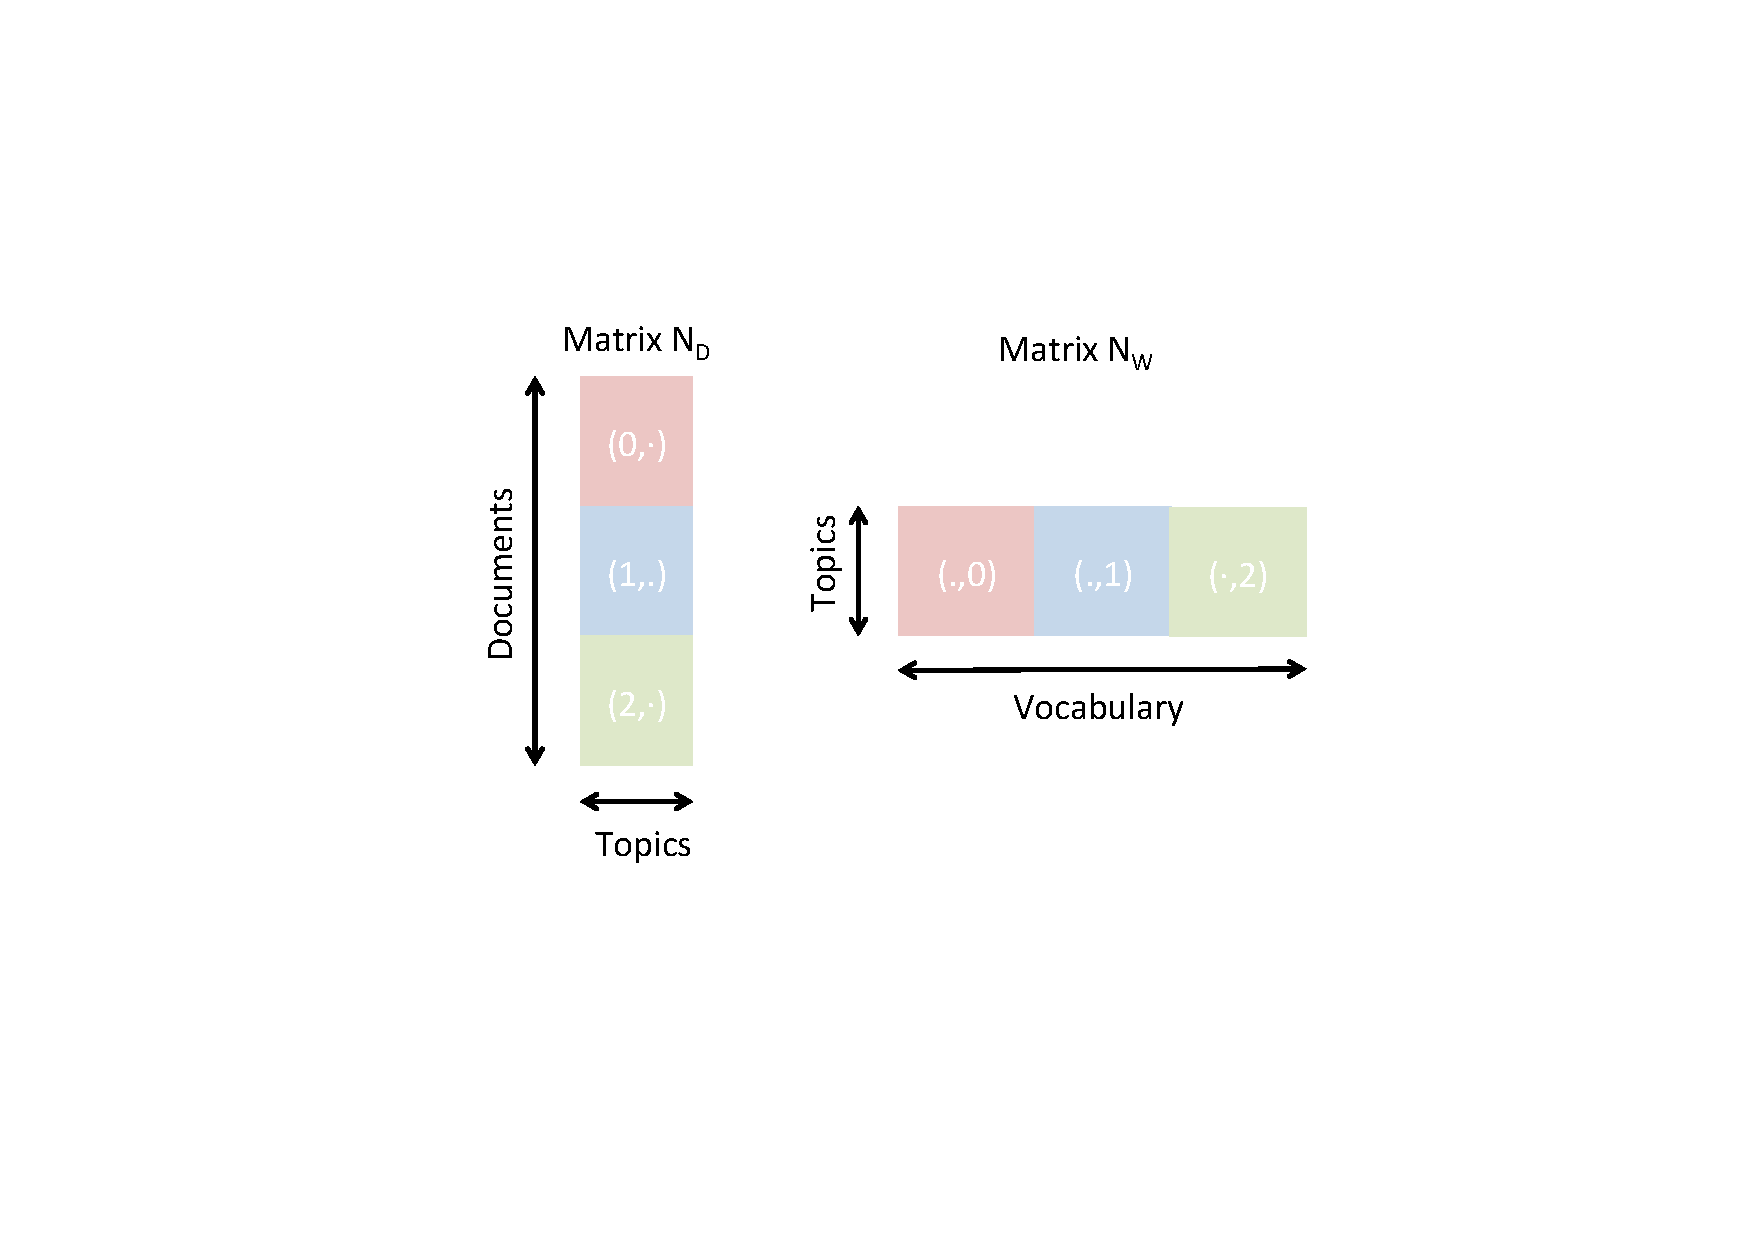
\includegraphics[width=0.8\linewidth,clip=true,trim=2cm 6cm 2cm 5cm]{figs/conflicts}
%%%	\end{figure}
%%%	
%%%	$$P(z_{d,n}=k, \bar{\mathbf Z}, {\mathbf W}|\alphabf, \eta)\propto \frac{(\bar n_d^k + \alpha_k) (\bar n_{w_{d,n}}^k + \eta)}{\sum_{r=1}^V \bar n_r^{k} + \eta}$$
%%%	
%%%	\begin{itemize}
%%%		\item Denominator needs use of all partitions of ${\mathbf N}_W$
%%%		\item Each processor updates these counts locally, and the sums are recalculated and broadcasted after each block processing
%%%	\end{itemize}
%%%
%%%\end{frame}
%%%
%%%
%%%
%%%\begin{frame}
%%%	\frametitle{Spark issues}
%%%	
%%%	\begin{figure}
%%%		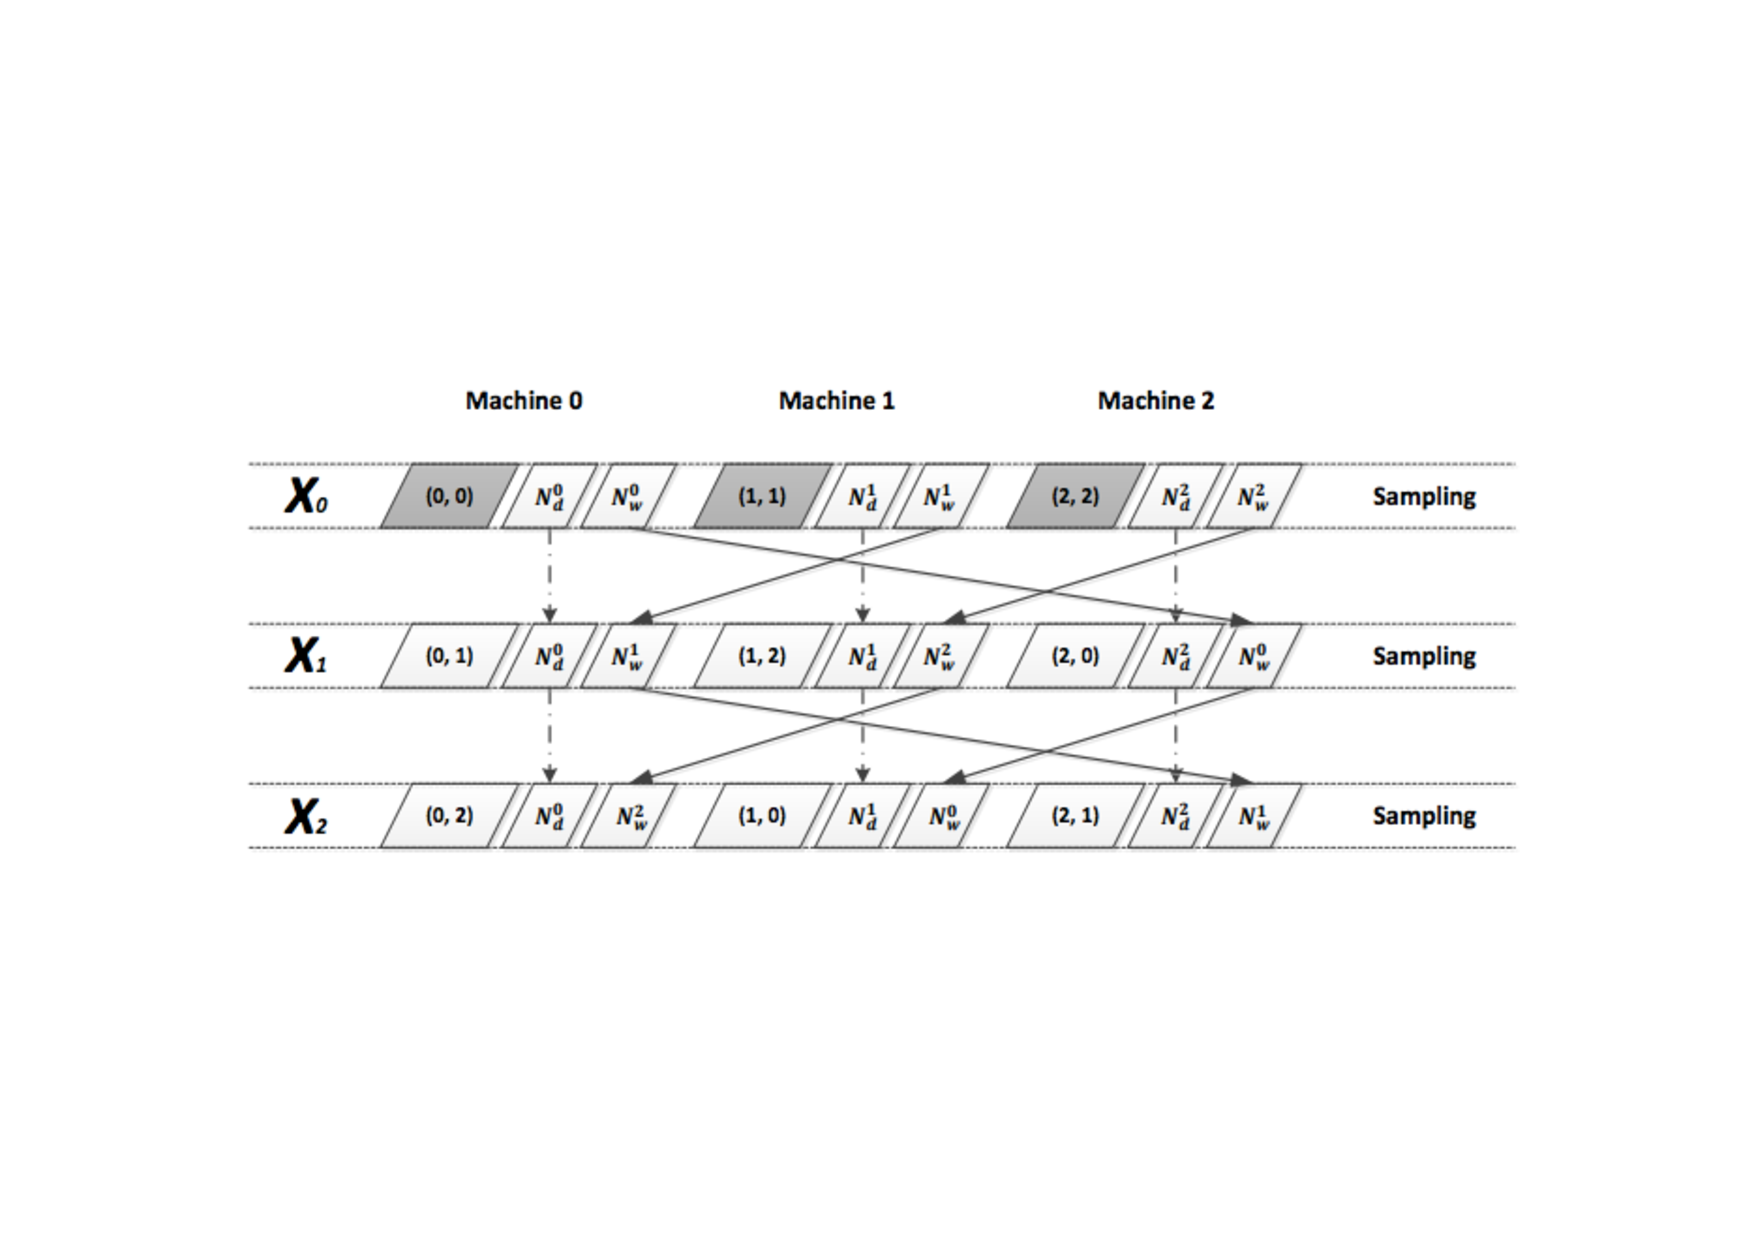
\includegraphics[width=0.8\linewidth,clip=true,trim=3cm 5.3cm 3cm 5.2cm]{figs/spark}
%%%	\end{figure}
%%%	
%%%	\begin{itemize}
%%%		\item Spark's resilient distributed datasets (RDD) can be used to store partitions that can be accessed from multiple processors
%%%		\item Spark is not good at operating more than two RDDs. Combine ${\bf Z}, {\mathbf N}_D,  {\mathbf N}_W$ in one RDD and split as necessary at each processor
%%%		{\begin{itemize} \item Time savings do not scale linearly with the number of processors\end{itemize}}
%%%		\item As we have seen, Gibbs sampling cannot be implemented exactly.
%%%		{\begin{itemize} \item Slower convergence \end{itemize}}
%%%	\end{itemize}
%%%	
%%%\end{frame}
%%%
%%%\begin{frame}
%%%	\frametitle{Results}
%%%	
%%%	\begin{figure}
%%%		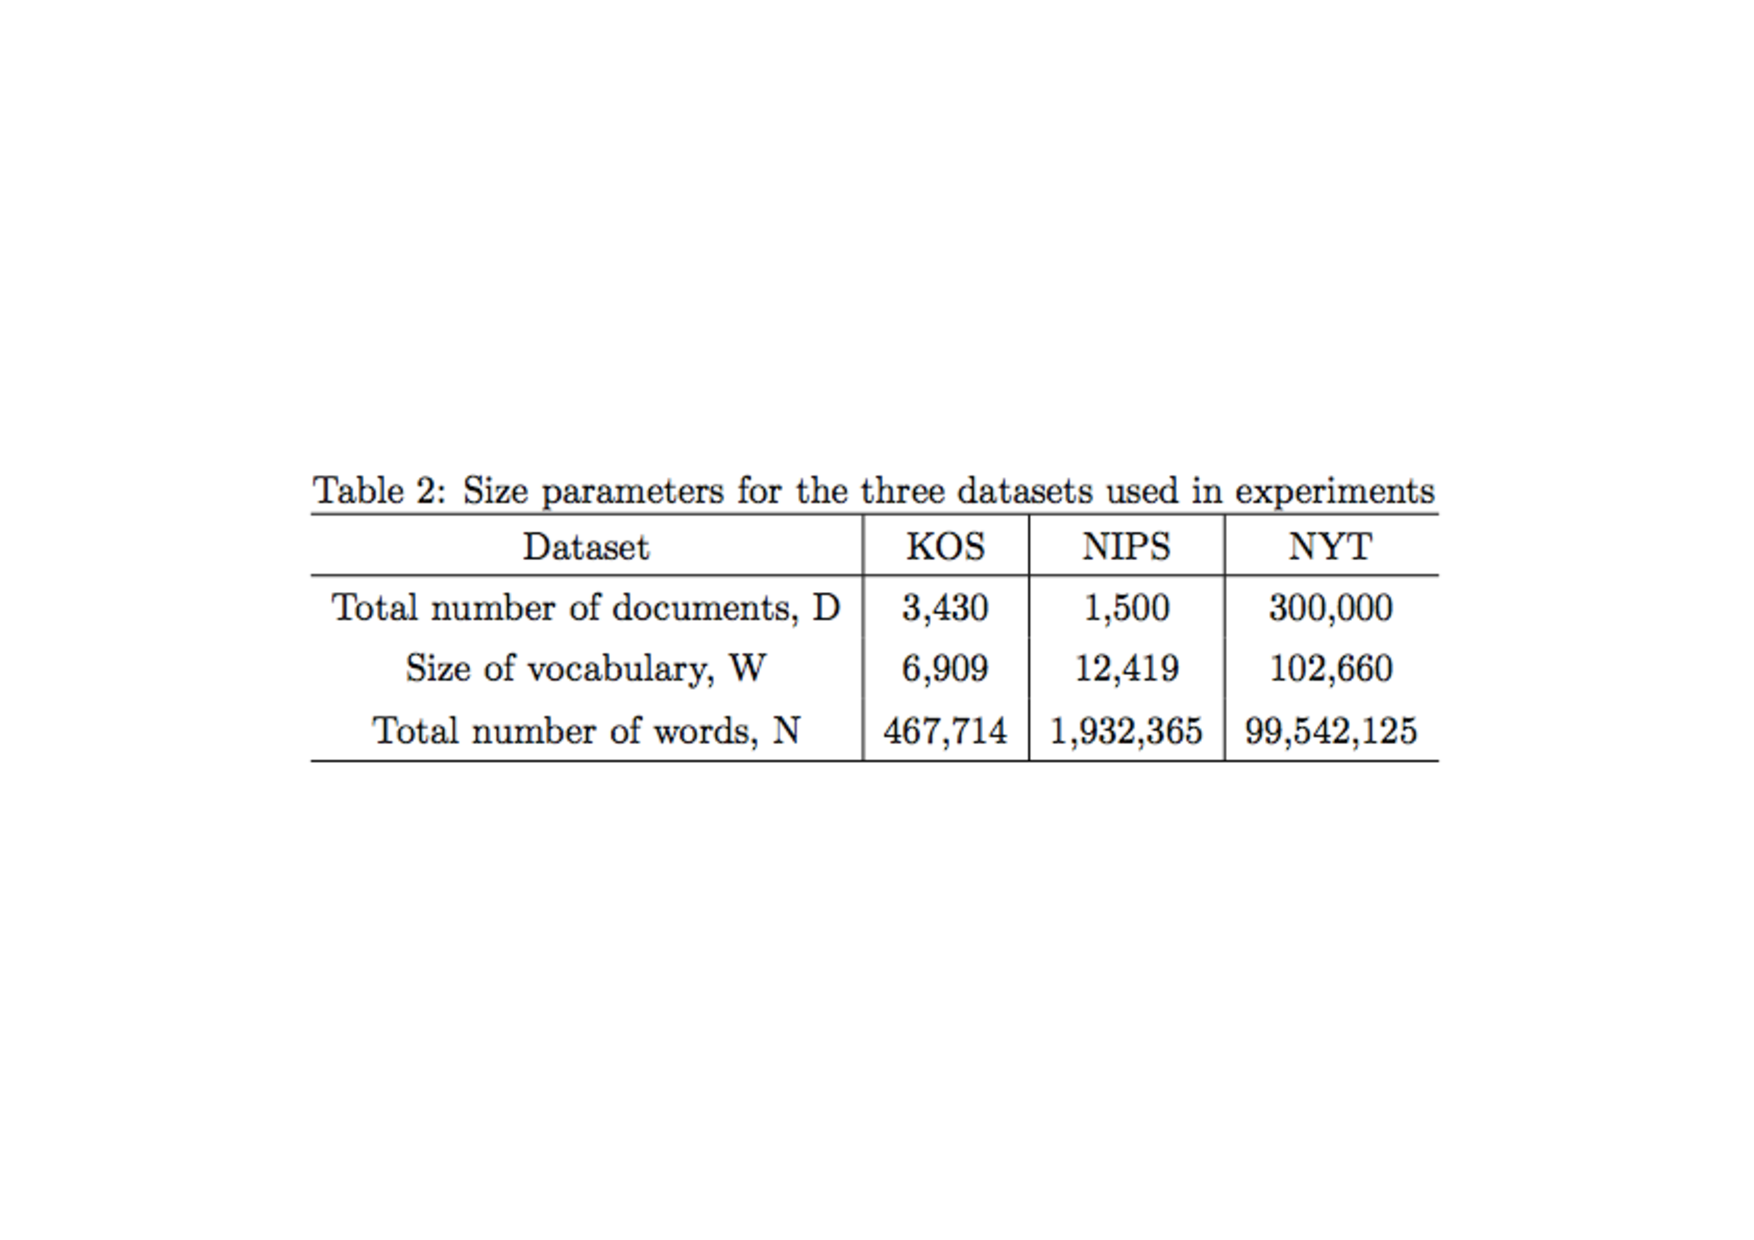
\includegraphics[width=1\linewidth,clip=true,trim=3cm 5.3cm 3cm 5.2cm]{figs/spark2}
%%%	\end{figure}
%%%	
%%%
%%%\end{frame}
%%%
%%%\begin{frame}
%%%	\frametitle{Results (II)}
%%%	
%%%	\begin{figure}
%%%		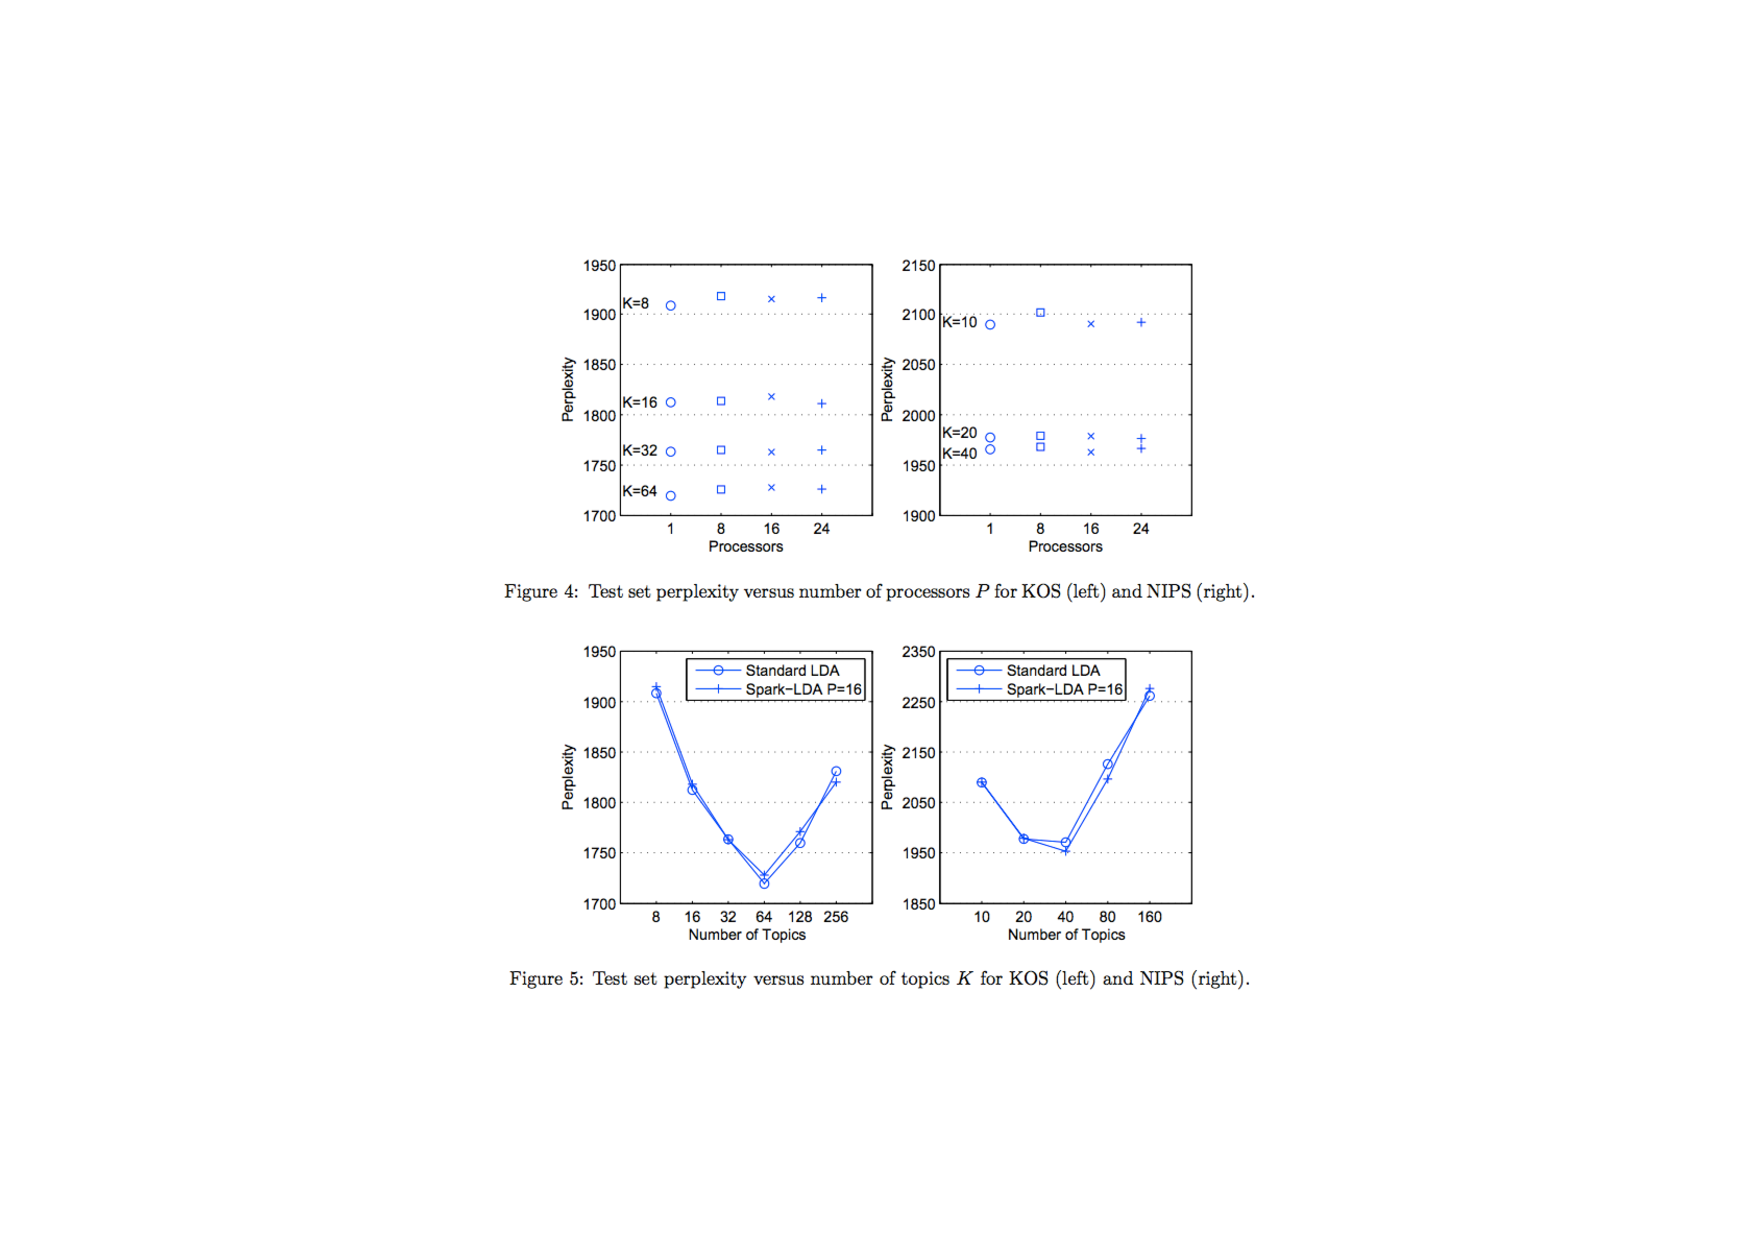
\includegraphics[width=0.9\linewidth,clip=true,trim=6cm 0cm 6cm 4cm]{figs/spark3}
%%%	\end{figure}
%%%	
%%%	
%%%\end{frame}
%%%
%%%\begin{frame}
%%%	\frametitle{Results (III)}
%%%	
%%%	\begin{figure}
%%%		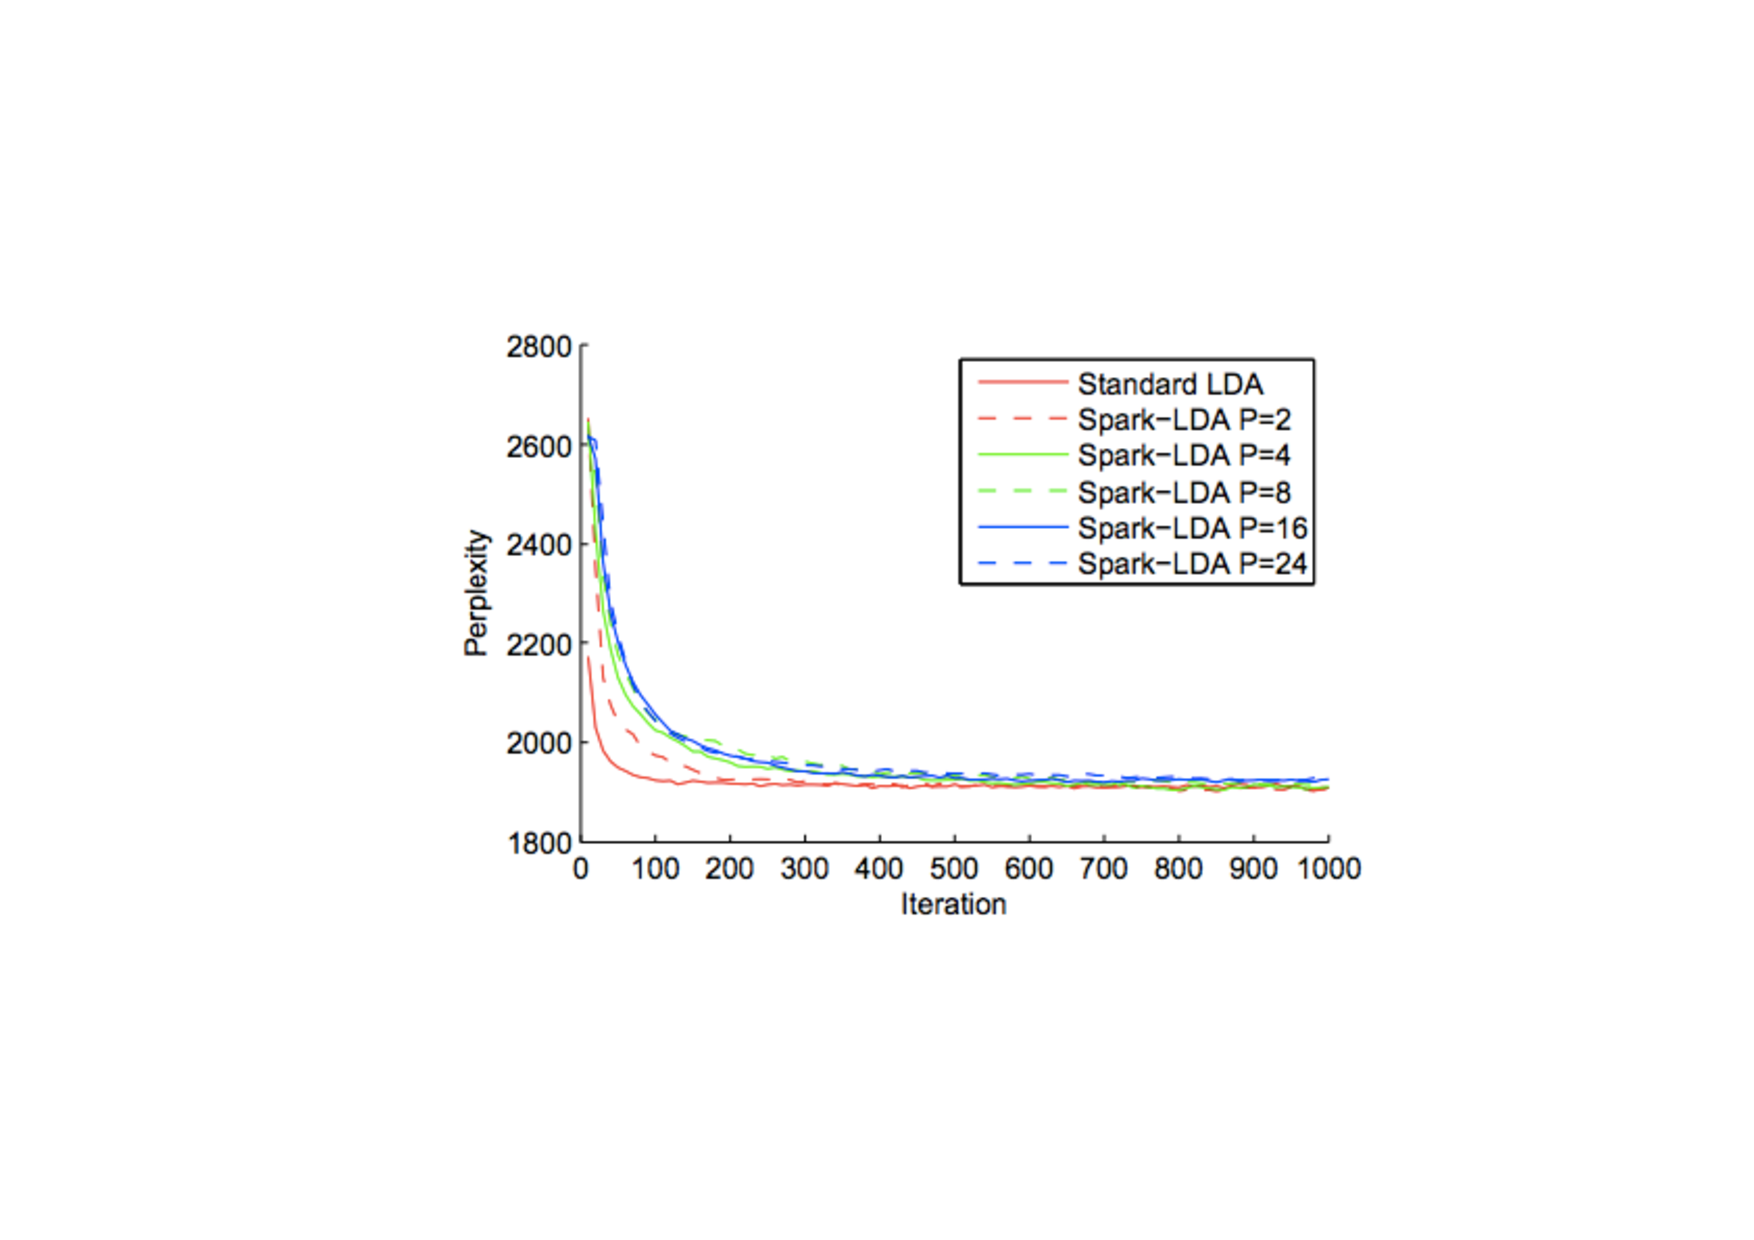
\includegraphics[width=0.9\linewidth,clip=true,trim=6cm 0cm 6cm 4cm]{figs/spark4}
%%%	\end{figure}
%%%	
%%%	
%%%\end{frame}
%%%
%%%
%%%\begin{frame}
%%%	\frametitle{Results (IV)}
%%%	
%%%	\begin{figure}
%%%		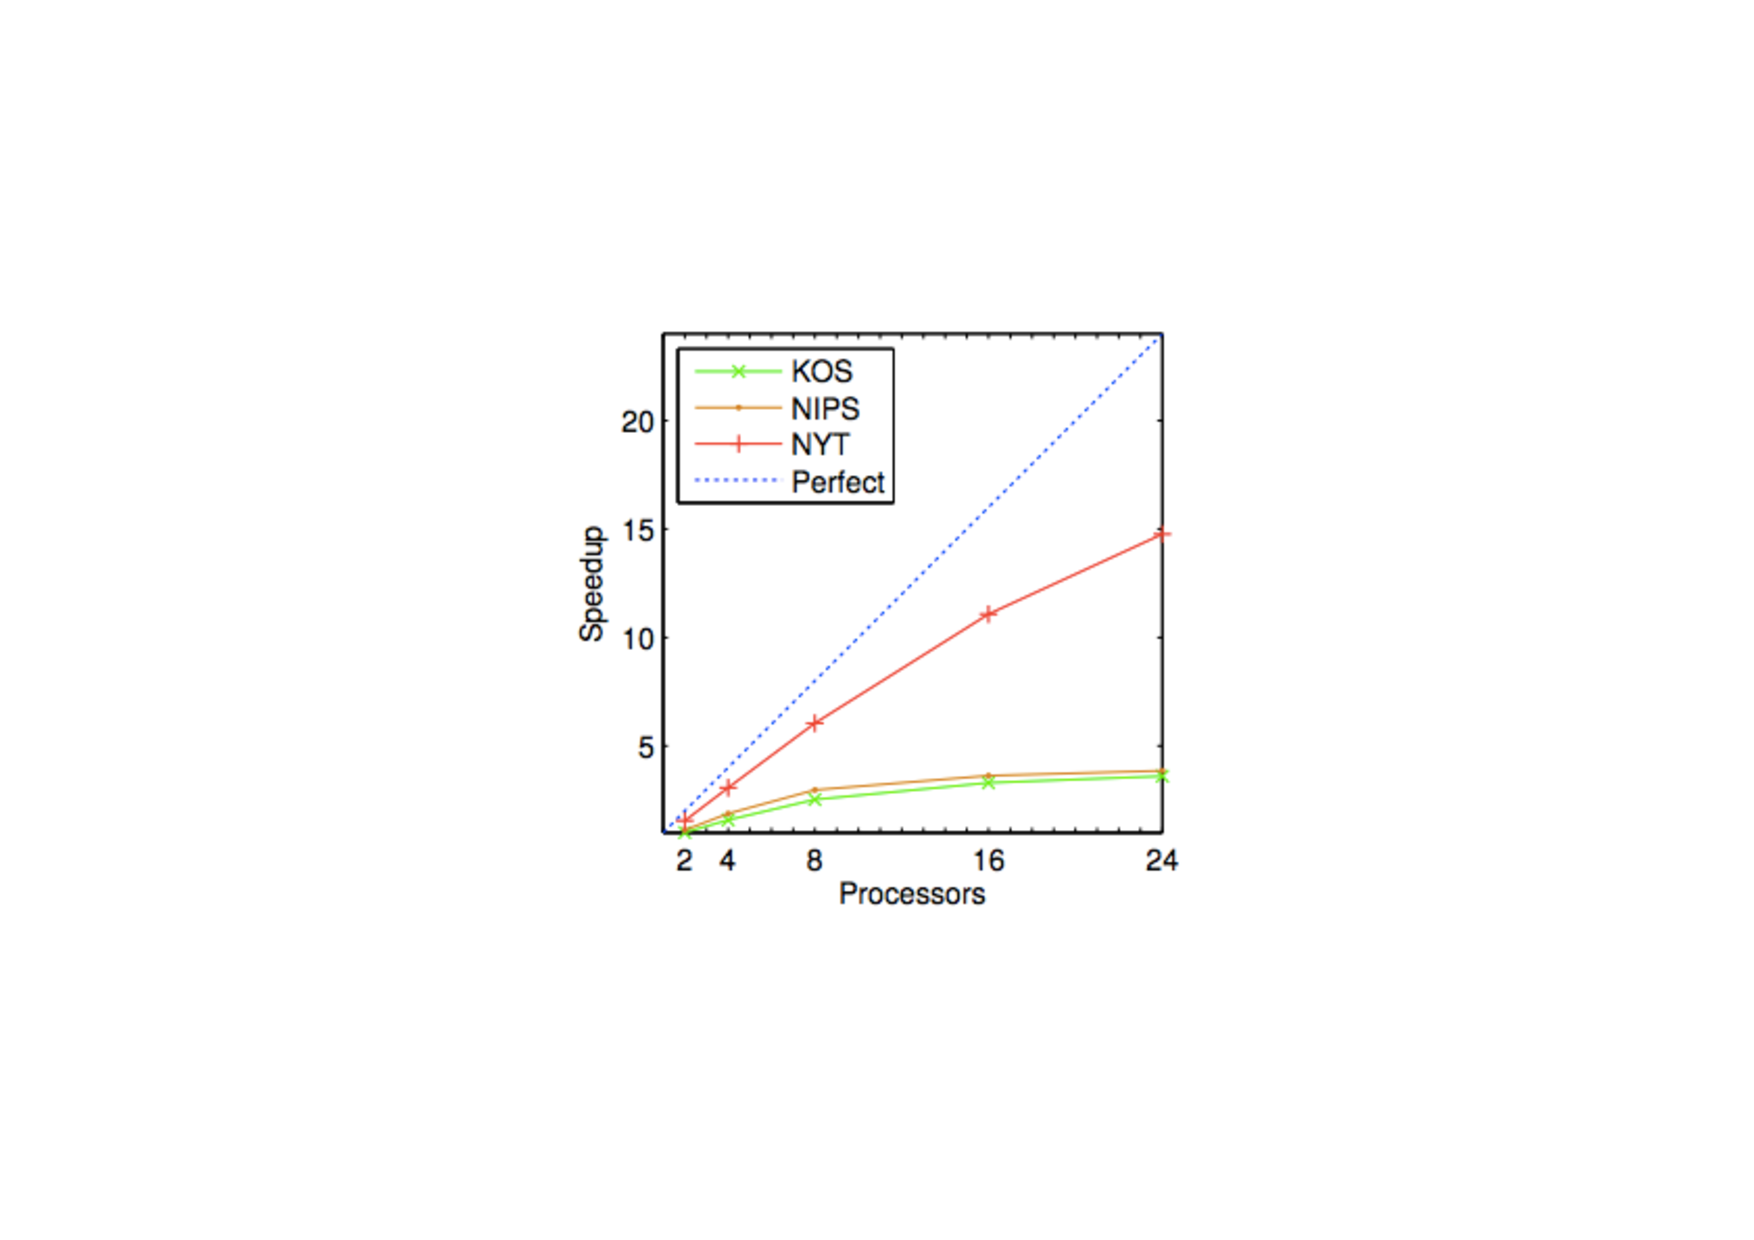
\includegraphics[width=0.9\linewidth,clip=true,trim=6cm 0cm 6cm 4cm]{figs/spark5}
%%%	\end{figure}
%%%	
%%%	
%%%\end{frame}
%%%
%%%%\begin{frame}
%%%%\frametitle{Paragraphs of Text}
%%%%Sed iaculis dapibus gravida. Morbi sed tortor erat, nec interdum arcu. Sed id lorem lectus. Quisque viverra augue id sem ornare non aliquam nibh tristique. Aenean in ligula nisl. Nulla sed tellus ipsum. Donec vestibulum ligula non lorem vulputate fermentum accumsan neque mollis.\\~\\
%%%%
%%%%Sed diam enim, sagittis nec condimentum sit amet, ullamcorper sit amet libero. Aliquam vel dui orci, a porta odio. Nullam id suscipit ipsum. Aenean lobortis commodo sem, ut commodo leo gravida vitae. Pellentesque vehicula ante iaculis arcu pretium rutrum eget sit amet purus. Integer ornare nulla quis neque ultrices lobortis. Vestibulum ultrices tincidunt libero, quis commodo erat ullamcorper id.
%%%%\end{frame}
%%%%
%%%%%------------------------------------------------
%%%%
%%%%\begin{frame}
%%%%\frametitle{Bullet Points}
%%%%\begin{itemize}
%%%%\item Lorem ipsum dolor sit amet, consectetur adipiscing elit
%%%%\item Aliquam blandit faucibus nisi, sit amet dapibus enim tempus eu
%%%%\item Nulla commodo, erat quis gravida posuere, elit lacus lobortis est, quis porttitor odio mauris at libero
%%%%\item Nam cursus est eget velit posuere pellentesque
%%%%\item Vestibulum faucibus velit a augue condimentum quis convallis nulla gravida
%%%%\end{itemize}
%%%%\end{frame}
%%%%
%%%%%------------------------------------------------
%%%%
%%%%\begin{frame}
%%%%\frametitle{Blocks of Highlighted Text}
%%%%\begin{block}{Block 1}
%%%%Lorem ipsum dolor sit amet, consectetur adipiscing elit. Integer lectus nisl, ultricies in feugiat rutrum, porttitor sit amet augue. Aliquam ut tortor mauris. Sed volutpat ante purus, quis accumsan dolor.
%%%%\end{block}
%%%%
%%%%\begin{block}{Block 2}
%%%%Pellentesque sed tellus purus. Class aptent taciti sociosqu ad litora torquent per conubia nostra, per inceptos himenaeos. Vestibulum quis magna at risus dictum tempor eu vitae velit.
%%%%\end{block}
%%%%
%%%%\begin{block}{Block 3}
%%%%Suspendisse tincidunt sagittis gravida. Curabitur condimentum, enim sed venenatis rutrum, ipsum neque consectetur orci, sed blandit justo nisi ac lacus.
%%%%\end{block}
%%%%\end{frame}
%%%%
%%%%%------------------------------------------------
%%%%
%%%%\begin{frame}
%%%%\frametitle{Multiple Columns}
%%%%\begin{columns}[c] % The "c" option specifies centered vertical alignment while the "t" option is used for top vertical alignment
%%%%
%%%%\column{.45\textwidth} % Left column and width
%%%%\textbf{Heading}
%%%%\begin{enumerate}
%%%%\item Statement
%%%%\item Explanation
%%%%\item Example
%%%%\end{enumerate}
%%%%
%%%%\column{.5\textwidth} % Right column and width
%%%%Lorem ipsum dolor sit amet, consectetur adipiscing elit. Integer lectus nisl, ultricies in feugiat rutrum, porttitor sit amet augue. Aliquam ut tortor mauris. Sed volutpat ante purus, quis accumsan dolor.
%%%%
%%%%\end{columns}
%%%%\end{frame}
%%%%
%%%%\begin{frame}
%%%%\frametitle{Table}
%%%%\begin{table}
%%%%\begin{tabular}{l l l}
%%%%\toprule
%%%%\textbf{Treatments} & \textbf{Response 1} & \textbf{Response 2}\\
%%%%\midrule
%%%%Treatment 1 & 0.0003262 & 0.562 \\
%%%%Treatment 2 & 0.0015681 & 0.910 \\
%%%%Treatment 3 & 0.0009271 & 0.296 \\
%%%%\bottomrule
%%%%\end{tabular}
%%%%\caption{Table caption}
%%%%\end{table}
%%%%\end{frame}
%%%%
%%%%%------------------------------------------------
%%%%
%%%%\begin{frame}
%%%%\frametitle{Theorem}
%%%%\begin{theorem}[Mass--energy equivalence]
%%%%$E = mc^2$
%%%%\end{theorem}
%%%%\end{frame}
%%%%
%%%%%------------------------------------------------
%%%%
%%%%\begin{frame}[fragile] % Need to use the fragile option when verbatim is used in the slide
%%%%\frametitle{Verbatim}
%%%%\begin{example}[Theorem Slide Code]
%%%%\begin{verbatim}
%%%%\begin{frame}
%%%%\frametitle{Theorem}
%%%%\begin{theorem}[Mass--energy equivalence]
%%%%$E = mc^2$
%%%%\end{theorem}
%%%%\end{frame}\end{verbatim}
%%%%\end{example}
%%%%\end{frame}
%%%%
%%%%%------------------------------------------------
%%%%
%%%%\begin{frame}
%%%%\frametitle{Figure}
%%%%Uncomment the code on this slide to include your own image from the same directory as the template .TeX file.
%%%%%\begin{figure}
%%%%%\includegraphics[width=0.8\linewidth]{test}
%%%%%\end{figure}
%%%%\end{frame}
%%%%
%%%%%------------------------------------------------
%%%%
%%%%\begin{frame}[fragile] % Need to use the fragile option when verbatim is used in the slide
%%%%\frametitle{Citation}
%%%%An example of the \verb|\cite| command to cite within the presentation:\\~
%%%%
%%%%This statement requires citation \cite{p1}.
%%%%\end{frame}
%%%%
%%%%%------------------------------------------------
%%%%
%%%%\begin{frame}
%%%%\frametitle{References}
%%%%\footnotesize{
%%%%\begin{thebibliography}{99} % Beamer does not support BibTeX so references must be inserted manually as below
%%%%\bibitem[Smith, 2012]{p1} John Smith (2012)
%%%%\newblock Title of the publication
%%%%\newblock \emph{Journal Name} 12(3), 45 -- 678.
%%%%\end{thebibliography}
%%%%}
%%%%\end{frame}
%%%%
%%%%%------------------------------------------------
%%%%
%%%%\begin{frame}
%%%%\Huge{\centerline{The End}}
%%%%\end{frame}
%%%
%%%%----------------------------------------------------------------------------------------

\end{document} 